\documentclass[twocolumn]{../../common/aa}
%\documentclass[referee]{aa}

\usepackage{graphicx}
\usepackage{amsmath,amsfonts,amssymb}
\usepackage{txfonts}
\usepackage{color}
\usepackage{natbib}
\usepackage{float}
%\usepackage{stfloats}
\usepackage{dblfloatfix}
\usepackage{afterpage}
\usepackage{ifthen}
\usepackage[morefloats=12]{morefloats}
\usepackage{placeins}
\usepackage{multicol}
\bibpunct{(}{)}{;}{a}{}{,}
\usepackage[switch]{lineno}
\definecolor{linkcolor}{rgb}{0.6,0,0}
\definecolor{citecolor}{rgb}{0,0,0.75}
\definecolor{urlcolor}{rgb}{0.12,0.46,0.7}
\PassOptionsToPackage{hyphens}{url}
\usepackage{url}
\usepackage[breaklinks, colorlinks, urlcolor=urlcolor,
    linkcolor=linkcolor,citecolor=citecolor,pdfencoding=auto]{hyperref}
\hypersetup{linktocpage}
\usepackage{bold-extra}
\usepackage{capt-of}


%\usepackage{xcolor}
%\usepackage[grid,
%  gridcolor=red!20,
%  subgridcolor=green!20,
%  gridunit=cm]{eso-pic}



%Planck style file, to be used with A&A style to produce Planck papers for publication.
%
% version 28 September 2010 --- useful macros --- CRL
% version 17 October 2010   --- first cut at important instrument values, from Daniele Mennella and
%                               Francois Bouchet, 13 October 2010 --- CRL
% version 18 October 2010   --- LFI FWHM changed to one value per feed, rather than M & S separately
%                               LFI FWHM uncertainties added for individual feeds.  Corrections made
%                               to LFI values. --- Andrea Zacchei
% version 24 October 2010   --- added to and corrected definitions.  No changes made to instrument
%                               quantities. --- CRL 
% version 31 October 2010   --- added definition of \muKHz. --- CRL
%
% version 15 November 2010  --- fixed conflict with aa.cls in definition of \endtable
%                               by naming the command below "\endPlancktable".  See section
%                               13.16 of the Style Guide.
%
% version 06 December 2010  --- Set up names with and without units.
%                               Add \allearlypapers command to ensure that all early papers are
%                               included in the reference list.
%                               Define macro for the name of the 4He JT cooler.
%
% version 07 December 2010  --- removed extraneous "planck2011-1.2" entry in \allearlypapers
%
% version 12 December 2010  --- added \endPlancktablewide command to set tablenotes to the full
%                               page width in the \begin{table*}...\end{table*} environment when
%                               the ``twocolumn'' option is specified in the \documentclass command.
%                               (It would be more elegant to extract the appropriate width from the
%                               aa.cls system at the time of execution, but that is buried more
%                               deeply in the system than I investigated.)
%
% version 05 January 2011   --- added unit \MJysr.  HFI performance values updated per FRB email
%                               01/05/2011 02:38-0800, and Brendan Crill email 01/05/2011 18:08 -0800.
%
% version 06 January 2011   --- changed \scriptscriptstyle primes to \scriptstyle, to better match the
%                               tx fonts used by A&A.
%
% version 07 January 2011   --- modified \allearlypapers to correspond with final early paper list.  
%                               Fixed 545 GHz center frequency.
%
% version 07 January 2011b  --- changed LFI white-noise sensitivity numbers to correct problem with units
%
% version 05 July 2011      --- added \Msol and \Lsol to get the symbols for solar mass and luminosity.
%                               Deleted previous definitions of \solar and \sol, which were equivalent
%                               to the new \Msol.
%
% version 16 August 2011    --- changed comments on \endPlancktable and \endPlancktablewide for clarity
%
% version 11 September 2011 --- changed definition of \tablenote to make footnote labels italic, as per A\&A
%
% version 26 April 2011     --- changed definition of \Planck to agree with what is said in the Style Guide (!)
%
% version 04 Dec 2013       --- included 2013 results references
%
% version 17 Jan 2014       --- included fix to bibtex file v4.3, i.e. \providecommand{\sorthelp}[1]{}
%
% version 26 Jul 2014       --- fixed incompatibility problem with aa.cls v8.0 and v8.2.  v8.2 should now be used
%                               for all Planck papers.
%                           --- fixed problem in definition of "\all2013resultspapers" that introduced a blanck
%                               into the reference to p06b.
%                           --- removed all the parameter definition stuff at the end.  We weren't using it, and
%                               it took up a lot of space.
%
% version 28 Jan 2015       --- added "\alltwentyfiftennresultspapers" and corrected "\all2013resultspapers" to
%                               "\all20thirteenresultspapers",
%
% Usage:  after the \documentclass[traditabstract]{aa} command in the La\TeX\ input file,
%         add this command:      \input Planck.tex


\def\setsymbol#1#2{\expandafter\def\csname #1\endcsname{#2}}
\def\getsymbol#1{\csname #1\endcsname}

%-----------------------------------------------------------------------
% Planck
%-----------------------------------------------------------------------
\def\Planck{\textit{Planck}}

%-----------------------------------------------------------------------
% The Planck Helium-4 JT cooler
%-----------------------------------------------------------------------
\def\HeJT{$^4$He-JT}

%-----------------------------------------------------------------------
% To include all Planck Early Results papers in the reference lists
%-----------------------------------------------------------------------
\def\allearlypapers{\nocite{planck2011-1.1, planck2011-1.3, planck2011-1.4, planck2011-1.5, planck2011-1.6, planck2011-1.7, planck2011-1.10, planck2011-1.10sup, planck2011-5.1a, planck2011-5.1b, planck2011-5.2a, planck2011-5.2b, planck2011-5.2c, planck2011-6.1, planck2011-6.2, planck2011-6.3a, planck2011-6.4a, planck2011-6.4b, planck2011-6.6, planck2011-7.0, planck2011-7.2, planck2011-7.3, planck2011-7.7a, planck2011-7.7b, planck2011-7.12, planck2011-7.13}}

%-----------------------------------------------------------------------
% To include all Planck 2013 Results papers in the reference lists
%-----------------------------------------------------------------------
\def\alltwentythirteenresultspapers{\nocite{planck2013-p01, planck2013-p02, planck2013-p02a, planck2013-p02d, planck2013-p02b, planck2013-p03, planck2013-p03c, planck2013-p03f, planck2013-p03d, planck2013-p03e, planck2013-p01a, planck2013-p06, planck2013-p03a, planck2013-pip88, planck2013-p08, planck2013-p11, planck2013-p12, planck2013-p13, planck2013-p14, planck2013-p15, planck2013-p05b, planck2013-p17, planck2013-p09, planck2013-p09a, planck2013-p20, planck2013-p19, planck2013-pipaberration, planck2013-p05, planck2013-p05a, planck2013-pip56, planck2013-p06b, planck2013-p01a}}

%-----------------------------------------------------------------------
% To include all Planck 2015 Results papers in the reference lists
%-----------------------------------------------------------------------
\def\alltwentyfifteenresultspapers{\nocite{planck2014-a01, planck2014-a03, planck2014-a04, planck2014-a05, planck2014-a06, planck2014-a07, planck2014-a08, planck2014-a09, planck2014-a11, planck2014-a12, planck2014-a13, planck2014-a14, planck2014-a15, planck2014-a16, planck2014-a17, planck2014-a18, planck2014-a19, planck2014-a20, planck2014-a22, planck2014-a24, planck2014-a26, planck2014-a28, planck2014-a29, planck2014-a30, planck2014-a31, planck2014-a35, planck2014-a36, planck2014-a37, planck2014-ES}}

%-----------------------------------------------------------------------
% Tables
%-----------------------------------------------------------------------
\newbox\tablebox    \newdimen\tablewidth
\def\leaderfil{\leaders\hbox to 5pt{\hss.\hss}\hfil}
%
% use the following definition of \endPlancktable for ApJ style notes to tables, set to the 
%         width of the table
% \def\endPlancktable{\tablewidth=\wd\tablebox 
%
% use the following definitions of \endPlancktable and \endPlancktablewide for A&A style notes 
% set to one-column  or full-page width, respectively
\def\endPlancktable{\tablewidth=\columnwidth 
    $$\hss\copy\tablebox\hss$$
    \vskip-\lastskip\vskip -2pt}
\def\endPlancktablewide{\tablewidth=\textwidth 
    $$\hss\copy\tablebox\hss$$
    \vskip-\lastskip\vskip -2pt}
\def\tablenote#1 #2\par{\begingroup \parindent=0.8em
    \abovedisplayshortskip=0pt\belowdisplayshortskip=0pt
    \noindent
    $$\hss\vbox{\hsize\tablewidth \hangindent=\parindent \hangafter=1 \noindent
    \hbox to \parindent{$^#1$\hss}\strut#2\strut\par}\hss$$
    \endgroup}
\def\doubleline{\vskip 3pt\hrule \vskip 1.5pt \hrule \vskip 5pt}

%-----------------------------------------------------------------------
% useful macros
%-----------------------------------------------------------------------
%
\def\L2{\ifmmode L_2\else $L_2$\fi}
%
\def\dtt{\Delta T/T}
\def\DeltaT{\ifmmode \Delta T\else $\Delta T$\fi}
\def\deltat{\ifmmode \Delta t\else $\Delta t$\fi}
\def\fknee{\ifmmode f_{\rm knee}\else $f_{\rm knee}$\fi}
\def\Fmax{\ifmmode F_{\rm max}\else $F_{\rm max}$\fi}
%
\def\solar{\ifmmode{\rm M}_{\mathord\odot}\else${\rm M}_{\mathord\odot}$\fi}
\def\Msolar{\ifmmode{\rm M}_{\mathord\odot}\else${\rm M}_{\mathord\odot}$\fi}
\def\Lsolar{\ifmmode{\rm L}_{\mathord\odot}\else${\rm L}_{\mathord\odot}$\fi}
%
\def\inv{\ifmmode^{-1}\else$^{-1}$\fi}
\def\mo{\ifmmode^{-1}\else$^{-1}$\fi}
\def\sup#1{\ifmmode ^{\rm #1}\else $^{\rm #1}$\fi}
\def\expo#1{\ifmmode \times 10^{#1}\else $\times 10^{#1}$\fi}
%
\def\,{\thinspace}
\def\lsim{\mathrel{\raise .4ex\hbox{\rlap{$<$}\lower 1.2ex\hbox{$\sim$}}}}
\def\gsim{\mathrel{\raise .4ex\hbox{\rlap{$>$}\lower 1.2ex\hbox{$\sim$}}}}
\let\lea=\lsim
\let\gea=\gsim
\def\simprop{\mathrel{\raise .4ex\hbox{\rlap{$\propto$}\lower 1.2ex\hbox{$\sim$}}}}
%
\def\deg{\ifmmode^\circ\else$^\circ$\fi}
\def\pdeg{\ifmmode $\setbox0=\hbox{$^{\circ}$}\rlap{\hskip.11\wd0 .}$^{\circ}
          \else \setbox0=\hbox{$^{\circ}$}\rlap{\hskip.11\wd0 .}$^{\circ}$\fi}
\def\arcs{\ifmmode {^{\scriptstyle\prime\prime}}
          \else $^{\scriptstyle\prime\prime}$\fi}
\def\arcm{\ifmmode {^{\scriptstyle\prime}}
          \else $^{\scriptstyle\prime}$\fi}
\newdimen\sa  \newdimen\sb
\def\parcs{\sa=.07em \sb=.03em
     \ifmmode \hbox{\rlap{.}}^{\scriptstyle\prime\kern -\sb\prime}\hbox{\kern -\sa}
     \else \rlap{.}$^{\scriptstyle\prime\kern -\sb\prime}$\kern -\sa\fi}
\def\parcm{\sa=.08em \sb=.03em
     \ifmmode \hbox{\rlap{.}\kern\sa}^{\scriptstyle\prime}\hbox{\kern-\sb}
     \else \rlap{.}\kern\sa$^{\scriptstyle\prime}$\kern-\sb\fi}
%
\def\ra[#1 #2 #3.#4]{#1\sup{h}#2\sup{m}#3\sup{s}\llap.#4}
\def\dec[#1 #2 #3.#4]{#1\deg#2\arcm#3\arcs\llap.#4}
\def\deco[#1 #2 #3]{#1\deg#2\arcm#3\arcs}
\def\rra[#1 #2]{#1\sup{h}#2\sup{m}}
%
\def\page{\vfill\eject}
\def\dots{\relax\ifmmode \ldots\else $\ldots$\fi}
%
%-----------------------------------------------------------------------
% units
%-----------------------------------------------------------------------
%
\def\WHzsr{\ifmmode $W\,Hz\mo\,sr\mo$\else W\,Hz\mo\,sr\mo\fi}
\def\mHz{\ifmmode $\,mHz$\else \,mHz\fi}
\def\GHz{\ifmmode $\,GHz$\else \,GHz\fi}
\def\mKs{\ifmmode $\,mK\,s$^{1/2}\else \,mK\,s$^{1/2}$\fi}
\def\muKs{\ifmmode \,\mu$K\,s$^{1/2}\else \,$\mu$K\,s$^{1/2}$\fi}
\def\muKRJs{\ifmmode \,\mu$K$_{\rm RJ}$\,s$^{1/2}\else \,$\mu$K$_{\rm RJ}$\,s$^{1/2}$\fi}
\def\muKHz{\ifmmode \,\mu$K\,Hz$^{-1/2}\else \,$\mu$K\,Hz$^{-1/2}$\fi}
\def\MJysr{\ifmmode \,$MJy\,sr\mo$\else \,MJy\,sr\mo\fi}
\def\MJysrmK{\ifmmode \,$MJy\,sr\mo$\,mK$_{\rm CMB}\mo\else \,MJy\,sr\mo\,mK$_{\rm CMB}\mo$\fi}
\def\microns{\ifmmode \,\mu$m$\else \,$\mu$m\fi}
\def\micron{\microns}
\def\muK{\ifmmode \,\mu$K$\else \,$\mu$\hbox{K}\fi}
\def\microK{\ifmmode \,\mu$K$\else \,$\mu$\hbox{K}\fi}
\def\muW{\ifmmode \,\mu$W$\else \,$\mu$\hbox{W}\fi}
\def\kms{\ifmmode $\,km\,s$^{-1}\else \,km\,s$^{-1}$\fi}
\def\kmsMpc{\ifmmode $\,\kms\,Mpc\mo$\else \,\kms\,Mpc\mo\fi}
%
%
%----------------------------------------------------------------------
% set up machinery to list Planck papers in roman numeral order.
%----------------------------------------------------------------------

\providecommand{\sorthelp}[1]{}


\def\WMAP{\emph{WMAP}}
\def\WMAPnine{\emph{WMAP9}}
\def\COBE{\emph{COBE}}
\def\wmap{\emph{WMAP}}
\def\planck{\emph{Planck}}
\def\Planck{\emph{Planck}}
\def\LCDM{$\Lambda$CDM}
\def\ffp{FFP6}
\def\unionmask{U73}
\def\nside{N_{\mathrm{side}}}

\def\healpix{\texttt{HEALPix}}
\def\commander{\texttt{Commander}}
\def\commanderone{\texttt{Commander1}}
\def\commandertwo{\texttt{Commander2}}
\def\commanderthree{\texttt{Commander3}}
\def\ruler{\texttt{Ruler}}
\def\comrul{\texttt{Commander-Ruler}}
\def\CR{\texttt{C-R}}
\def\nilc{\texttt{NILC}}
\def\gnilc{\texttt{GNILC}}
\def\sevem{\texttt{SEVEM}}
\def\smica{\texttt{SMICA}}
\def\CamSpec{\texttt{CamSpec}}
\def\Plik{\texttt{Plik}}
\def\XFaster{\texttt{XFaster}}
\def\sroll2{\texttt{SRoll2}}

\renewcommand{\d}[0]{\vec{d}}
\renewcommand{\t}[0]{\vec{t}}
\newcommand{\A}[0]{\mathrm{A}}
\newcommand{\B}[0]{\mathrm{B}}
\newcommand{\Y}[0]{\tens{Y}}
\newcommand{\n}[0]{\vec{n}}
\newcommand{\red}[0]{\color{red}}
\newcommand{\green}[0]{\color{green}}
\newcommand{\s}[0]{\vec{s}}
%\renewcommand{\a}[0]{\vec{a}}
\newcommand{\m}[0]{\vec{m}}
\newcommand{\f}[0]{\vec{f}}
\newcommand{\F}[0]{\tens{F}}
\newcommand{\T}[0]{\tens{T}}
\newcommand{\Cp}[0]{\tens{C}}
\renewcommand{\L}[0]{\tens{L}}
\newcommand{\g}[0]{\vec{g}}
\newcommand{\N}[0]{\tens{N}}
\newcommand{\M}[0]{\tens{M}}
\newcommand{\iN}[0]{\tens{N}^{-1}}
\newcommand{\iM}[0]{\tens{M}^{-1}}
\newcommand{\w}[0]{\vec{w}}
\renewcommand{\S}[0]{\tens{S}}
\renewcommand{\r}[0]{\vec{r}}
\renewcommand{\u}[0]{\vec{u}}
\newcommand{\q}[0]{\vec{q}}
\renewcommand{\v}[0]{\vec{v}}
\renewcommand{\P}[0]{\tens{P}}
\newcommand{\dt}[0]{d_t}
\newcommand{\di}[0]{d_i}
\newcommand{\nt}[0]{n_t}
\newcommand{\st}[0]{s_t}
\newcommand{\mt}[0]{m_t}
\newcommand{\ft}[0]{f_t}
\newcommand{\Te}[0]{T_{\rm e}}
\newcommand{\EM}[0]{\rm EM}
\newcommand{\mathsc}[1]{{\normalfont\textsc{#1}}}
\newcommand{\hi}{\ensuremath{\mathsc {Hi}}}
\newcommand{\bpbold}{\bfseries{\scshape{BeyondPlanck}}}
\newcommand{\BP}{\textsc{BeyondPlanck}}
\newcommand{\bp}{\textsc{BeyondPlanck}}
\newcommand{\cosmoglobe}{\textsc{Cosmoglobe}}
\newcommand{\Cosmoglobe}{\textsc{Cosmoglobe}}
\newcommand{\lfi}[0]{LFI}
\newcommand{\hfi}[0]{HFI}
\newcommand{\npipe}[0]{\texttt{NPIPE}}
\newcommand{\K}[0]{\textit K}
\newcommand{\Ka}[0]{\textit{Ka}}
\newcommand{\Q}[0]{\textit Q}
\newcommand{\V}[0]{\textit V}
\newcommand{\W}[0]{\textit W}
\newcommand{\e}{\mathrm e}
\newcommand{\cvar}{\ensuremath{c(\vartheta, \varphi, \psi)}}

\usepackage[T1]{fontenc}


\def\bC{\tens{C}}
\def\ba{\vec{a}}
\def\ncha{N_\mathrm{cha}}
\def\nfg{N_\mathrm{fg}}

\newcommand{\ncorr}{\vec n_\mathrm{corr}}
\newcommand{\Dbp}{\Delta_\mathrm{bp}}

%\modulolinenumbers[5]
%\linenumbers

\newcommand{\includegraphicsdpi}[3]{
    \pdfimageresolution=#1  % Change the dpi of images
    \includegraphics[#2]{#3}
    \pdfimageresolution=72  % Change it back to the default
}

\renewcommand{\topfraction}{1.0}	% max fraction of floats at top
    \renewcommand{\bottomfraction}{1.0}	% max fraction of floats at bottom
    %   Parameters for TEXT pages (not float pages):
    \setcounter{topnumber}{2}
    \setcounter{bottomnumber}{2}
    \setcounter{totalnumber}{4}     % 2 may work better
    \setcounter{dbltopnumber}{2}    % for 2-column pages
    \renewcommand{\dbltopfraction}{0.9}	% fit big float above 2-col. text
    \renewcommand{\textfraction}{0.04}	% allow minimal text w. figs
    %   Parameters for FLOAT pages (not text pages):
    \renewcommand{\floatpagefraction}{0.9}	% require fuller float pages
	% N.B.: floatpagefraction MUST be less than topfraction !!
    \renewcommand{\dblfloatpagefraction}{0.9}	% require fuller float pages

\def\adj{^{\dagger}}
\def\tp{^{\rm T}}
\def\inv{^{-1}}
\def\lm{{\ell m}}

\begin{document}

\title{\bfseries{\Cosmoglobe\ DR1. III. First full-sky model of polarized synchrotron\\ emission from all \WMAP\ and \Planck\ LFI data}}
%This author list corresponds to \title{Author list for L04\_CMB\_Foregrounds\_Extraction}
%Prepared by M. Lopez-Caniego (Marcos.Lopez.Caniego@sciops.esa.int), ESAC/ESA
%This version is from Thu Jul 12 18:11:48 2018 CET
%\subtitle{There are 152 co-authors in this list}
\newcommand{\oslo}[0]{1}
\newcommand{\iiabangalore}[0]{2}

\author{\small
D.~J.~Watts\inst{\ref{uio}}\thanks{Corresponding author: D.~J.~Watts; \url{duncanwa@astro.uio.no}}
\and
A.~Basyrov\inst{\ref{uio}}
\and
H.~T.~Ihle\inst{\ref{uio}}
\and
S.~Paradiso\inst{\ref{waterloo}}
\and
F.~Rahman\inst{\ref{iiabangalore}}
\and
H.~Thommesen\inst{\ref{uio}}
\and
M.~Bersanelli\inst{\ref{milan}}
\and
L.~A.~Bianchi\inst{\ref{milan}}
\and
M.~Brilenkov\inst{\ref{uio}}
\and
L.~P.~L.~Colombo\inst{\ref{milan}}
\and
H.~K.~Eriksen\inst{\ref{uio}}
\and
J.~R.~Eskilt\inst{\ref{uio},\ref{imperial}}
\and
K.~S.~F.~Fornazier\inst{\ref{saopaulo}}
\and
C.~Franceschet\inst{\ref{milan}}
\and
U.~Fuskeland\inst{\ref{uio}}
\and
M.~Galloway\inst{\ref{uio}}
\and
E.~Gjerl\o w\inst{\ref{uio}}
\and
B.~Hensley\inst{\ref{princeton}}
\and
L.~T.~Hergt\inst{\ref{ubc}}
\and
D.~Herman\inst{\ref{uio}}
\and
G.~A.~Hoerning\inst{\ref{saopaulo}}
\and
K.~Lee\inst{\ref{uio}}
\and
J.~G.~S.~Lunde\inst{\ref{uio}}
\and
A.~Marins\inst{\ref{saopaulo},\ref{ustofc}}
\and
S.~K.~Nerval\inst{\ref{dunlap1},\ref{dunlap2}}
\and
S.~K.~Patel\inst{\ref{iit_bhu}}
\and
M.~Regnier\inst{\ref{apc}}
\and
M.~San\inst{\ref{uio}}
\and
S.~Sanyal\inst{\ref{iit_bhu}}
\and
N.-O.~Stutzer\inst{\ref{uio}}
\and
A.~Verma\inst{\ref{iit_bhu}}
\and
I.~K.~Wehus\inst{\ref{uio}}
\and
Y.~Zhou\inst{\ref{berkeley}}
}
\institute{\small
Institute of Theoretical Astrophysics, University of Oslo, Blindern, Oslo, Norway\label{uio}
\and
Waterloo Centre for Astrophysics, University of Waterloo, Waterloo, ON N2L 3G1, Canada\label{waterloo}
\and
Indian Institute of Astrophysics, Koramangala II Block, Bangalore, 560034, India\label{iiabangalore}
\and
Dipartimento di Fisica, Università degli Studi di Milano, Via Celoria, 16, Milano, Italy\label{milan}
\and
Imperial Centre for Inference and Cosmology, Department of Physics, Imperial College London, Blackett Laboratory, Prince Consort Road, London SW7 2AZ, United Kingdom\label{imperial}
\and
Instituto de Física, Universidade de São Paulo - C.P. 66318, CEP: 05315-970, São Paulo, Brazil\label{saopaulo}
\and
Department of Astrophysical Sciences, Princeton University, 4 Ivy Lane, Princeton, NJ 08540\label{princeton}
\and
Department of Physics and Astronomy, University of British Columbia, 6224 Agricultural Road, Vancouver BC, V6T1Z1, Canada\label{ubc}
\and
Department of Astronomy,  University of Science and Technology of China, Hefei, China\label{ustofc}
\and
David A. Dunlap Department of Astronomy \& Astrophysics, University of Toronto, 50 St. George Street, Toronto, ON M5S 3H4, Canada\label{dunlap1}
\and
Dunlap Institute for Astronomy \& Astrophysics, University of Toronto, 50 St. George Street, Toronto, ON M5S 3H4, Canada\label{dunlap2}
\and
Department of Physics, Indian Institute of Technology (BHU), Varanasi - 221005, India\label{iit_bhu}
\and
Laboratoire Astroparticule et Cosmologie (APC), Université Paris-Cité, Paris, France\label{apc}
\and
Department of Physics, UC Berkeley\label{berkeley}
}

 %\author{V.~Arsenijevic\inst{\ref{inst1}}\and S.~Fabbro\inst{\ref{inst2}}\and
%A.~M.~Mour\~ao\inst{\ref{inst3}}\and A.~J.~Rica da Silva\inst{\ref{inst1}}}
%
%\institute{Multidisciplinar de Astrof\'{\i}sica, IST, Avenida Rovisco Pais, 1049
%Lisbon, Portugal\email{...}\label{inst1} \and < Multidisciplinar de Astrof\'{\i}sica, IST, Avenida Rovisco Pais, 1049 Lisbon, Portugal\email{...}\label{inst2}
%\and
%Multidisciplinar de Astrof\'{\i}sica, IST, Avenida Rovisco Pais, 1049
%Lisbon, Portugal\email{...}\label{inst3}
%} 

\authorrunning{Watts et al.}
\titlerunning{\cosmoglobe\ Polarized Synchrotron Analysis}

\abstract{
	We present the first model of full-sky polarized synchrotron emission that is derived from all \WMAP\ and \Planck\ LFI frequency maps. The basis of this analysis is the set of end-to-end reprocessed \cosmoglobe\ Data Release 1 sky maps presented in a companion paper, which have significantly lower instrumental systematics than the legacy products from each experiment. We find that the resulting polarized synchrotron amplitude map has an average noise rms of $3.2\,\mathrm{\mu K}$ at 30\,GHz and $2^{\circ}$ FWHM, which is 30\,\% lower than the recently released \BP\ model that included only LFI+\WMAP\ \Ka--\V\ data, and 29\,\% lower than the raw \WMAP\ \K-band sensitivity. The mean $EE/BB$ power spectrum ratio is $0.46\pm0.03$, with amplitudes consistent with those measured previously by  \Planck\ and QUIJOTE. Assuming a power law model for the synchrotron spectral energy distribution, and using the T-T plot method, we find a full-sky inverse noise-variance weighted mean of $\beta_{\mathrm{s}}=-3.07\pm0.07$ between \cosmoglobe\ DR1 \K-band and 30\,GHz, in good agreement with previous estimates. In summary, the novel \cosmoglobe\ DR1 synchrotron model is both more sensitive and systematically cleaner than similar previous models, and it has a more complete error description that is defined by a set of Monte Carlo posterior samples. We believe that these products are preferable for all synchrotron-related scientific applications than previous products compared to previous \Planck\ and \WMAP\ products, including simulation, forecasting and component separation. 
}

\keywords{ISM: general -- Cosmology: observations, polarization,
    cosmic microwave background, diffuse radiation -- Galaxy:
    general}

\maketitle

%\hypersetup{linkcolor=black}
\tableofcontents
%\hypersetup{linkcolor=red} 




\section{Introduction}
\label{sec:introduction}

Understanding the polarization of the cosmic microwave background (CMB) is a primary focus of observational cosmology in the coming decades. Following the success of the satellite-based \COBE\ \citep{smoot:1992,mather:1994,hauser:1998}, \textit{Wilkinson Microwave Anisotropy Probe} (\WMAP) \citep{bennett2012}, and \Planck\ \citep{planck2016-l01} experiments, as well as sub-orbital experiments including BICEP \citep{bicep2021}, ACT \citep{actDR6_lensing}, CLASS \citep{eimer2023}, SPIDER \citep{spider21}, and many others, the future \textit{LiteBIRD} satellite \citep{litebird2022} and ground-based Simons Observatory \citep{SO2019} and CMB-S4 \citep{cmbs4} experiments will create the most sensitive maps of the polarized sky yet, providing the most stringent constraints on primordial gravitational waves.

In the past decade, uncertainties on cosmological constraints have been limited not only by instrumental sensitivity, but by incomplete knowledge of the sky itself. Uncertainty in the sky model has been mitigated by designing experiments with broad frequency coverage, such as \WMAP\ \citep{bennett2012} and \Planck\ \citep{planck2016-l01}, or analyzing maps from different experiments jointly (e.g., \citealp{dmr}, \citealp{bennett2012}, \citealp{planck2014-a12}, and \citealp{pb2015}, among many others).
A major impediment to joint analyses is the difficulty of combining data with different survey strategies and incompletely characterized systematics. In order to maximize scientific throughput, one must either design an experiment that can characterize every relevant observable on its own, or jointly analyze different datasets in the same joint framework.

The \bp\ project achieved such joint analysis by combining external data, specifically, the Haslam 408\,MHz map \citep{haslam1982}, \WMAP\ \Ka--\V\ bands, \Planck\ 353\,GHz in polarization, and \Planck\ 857\,GHz in intensity, while analyzing the \Planck\ 30, 44, and 70 GHz time-ordered data (TOD) \citep{bp01}.
The \Planck\ LFI experiment showed that raw detector sensitivity was not enough to obtain high-fidelity sky maps; \citet{planck2016-l02} found that the detector gain solution depended on the assumed polarization and intensity of the sky. To break this circular dependency, the \bp\ framework solved for the intrinsic sky signal and instrumental parameters iteratively, providing an accurate model of the entire system with full error propagation. By leveraging the external \WMAP, Haslam, and \Planck\ HFI  data, \bp\ was able to create \Planck\ LFI maps of cosmological quality at all frequency channels, while generating a robust model of the foreground sky.

The \cosmoglobe\ project\footnote{\url{cosmoglobe.uio.no}} has generalized the \bp\ analysis by additionally processing \WMAP\ \K--\W-band TOD jointly with \Planck\ LFI TOD. This framework, fully described in \citet{bp17} and \cite{watts2023_dr1},
not only improved the quality of the \WMAP\ maps themselves, but provided the most robust full-sky model of low frequency polarized emission available to date. In particular, poorly-measured modes due to transmission imbalance \citep{jarosik2007} have been effectively marginalized over, in large part due to the use of a global sky model that was not used in the fiducial \WMAP\ analyses. The removal of poorly measured modes alone will improve Galactic modelling for years to come, as the current state-of-the-art models use \WMAP\ \K-band (23\,GHz) maps as polarized synchrotron templates for modeling of synchrotron without any mitigation of the poorly-measured modes \citep{delabrouille2012,pysm2,pysm3}.

In order to make use of the synchrotron model, we require robust estimates of the spectral behavior. Fundamental properties of synchrotron, such as the spectral index as a function of frequency, spatial decorrelation, and even the functional form of the spectral energy distribution (SED), are yet to be fully characterized observationally. Modern attempts have been frustrated by the lack of high signal-to-noise data; \citet{deBelsunce:2022}, for example, find spectral indices ranging from $-5$ to $-1$, discrepant with predictions from direct measurements of the cosmic ray energy spectrum of 2--3 \citep{rybicki,orlando2013,neronov2017}, largely due to fitting too many parameters to data with too low signal-to-noise ratio. Such analyses can be greatly improved by combining complementary data sets.

While the combination of as many datasets as possible would help to constrain polarized synchrotron's large-scale properties, long-standing discrepancies between existing datasets complicate this. As shown by, for example, \citet{planck2014-a12} and \citet{weiland:2018}, there are discrepancies in the polarization measurements of \WMAP\ and \Planck, partially due known instrumental effects \citep{bennett2012,planck2016-l02}. \citet{bp01} largely resolved these issues for LFI, while \citet{bp17} removed the poorly measured modes in \WMAP. In the first \cosmoglobe\ data release, of which this paper is a part, \citet{watts2023_dr1} demonstrated that the polarized maps resulting from these two experiments are consistent at the noise level after recalibrating both experiments jointly. At the same time, the new maps must be validated by a variety of analysis methods. As noted in, for example, \citet{weiland:2022}, simply using a different analysis pipeline can result in different estimations of the underlying frequency map. As such, we take care to appopriately marginalize over instrumental effects in our spectral analysis, and attempt to find the physical reason for the differences between different pipelines.

With these longstanding discrepancies addressed, the main goal of the current paper is to derive the highest signal-to-noise ratio model of polarized synchrotron emission from \Planck\ and \WMAP\ data published to date, including both amplitude and spectral index parameters. This work is organized as follows. In Sect.~\ref{sec:data}, we provide a brief overview of the data products and the \cosmoglobe\ data processing. Section~\ref{sec:pol_amp} discusses the polarized amplitude of the \cosmoglobe\ synchrotron model, its overall uncertainty, and the power spectrum properties compared to external products. Section~\ref{sec:specvar} estimates the synchrotron spectral index using both the T-T plot method and Gibbs sampling using \commander, followed by discussions and conclusions in Sect.~\ref{sec:conclusion}.

%In this work, we will use the \WMAP\ and LFI frequency maps generated in the \cosmoglobe\ DR1 analysis. 

%We perform three separate analyses; a map and power spectrum-based analysis of the synchrotron amplitude, linear correlation within regions (T-T plots), and per-pixel Gibbs sampling.





\section{Data products}
\label{sec:data}

\begin{figure*}
	\centering
	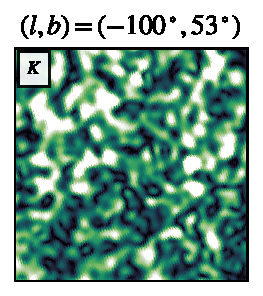
\includegraphics[width=0.2\textwidth]{figures/K_square.pdf}
	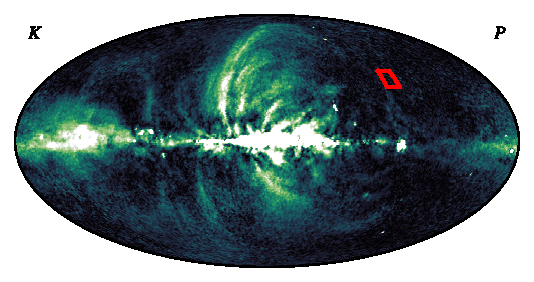
\includegraphics[width=0.35\textwidth]{figures/Kband_polint.pdf}
	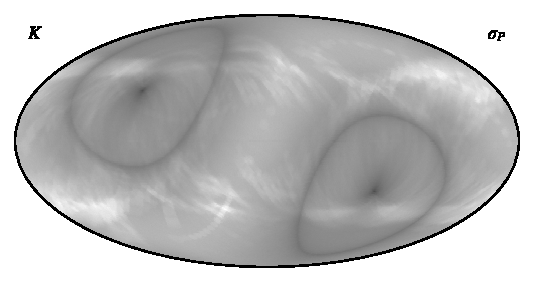
\includegraphics[width=0.35\textwidth]{figures/Kband_sigmaP.pdf}\\
	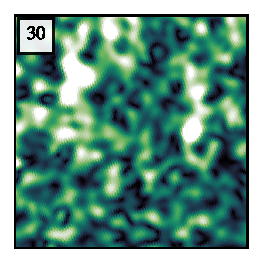
\includegraphics[width=0.2\textwidth]{figures/30_square.pdf}
	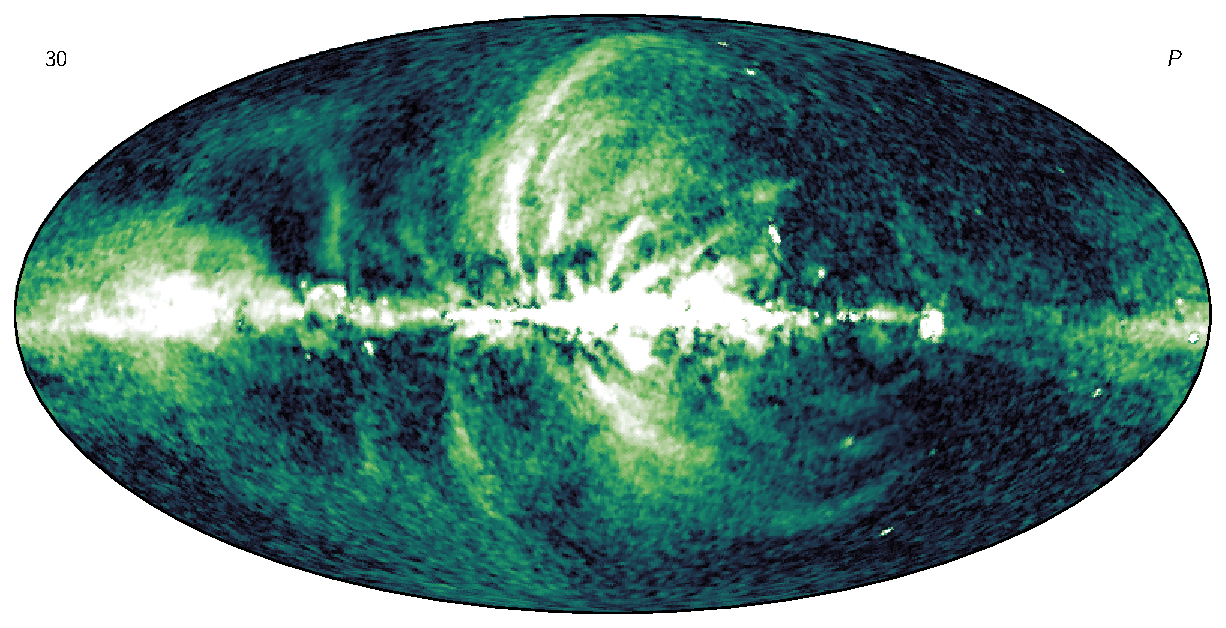
\includegraphics[width=0.35\textwidth]{figures/30GHz_polint.pdf}
	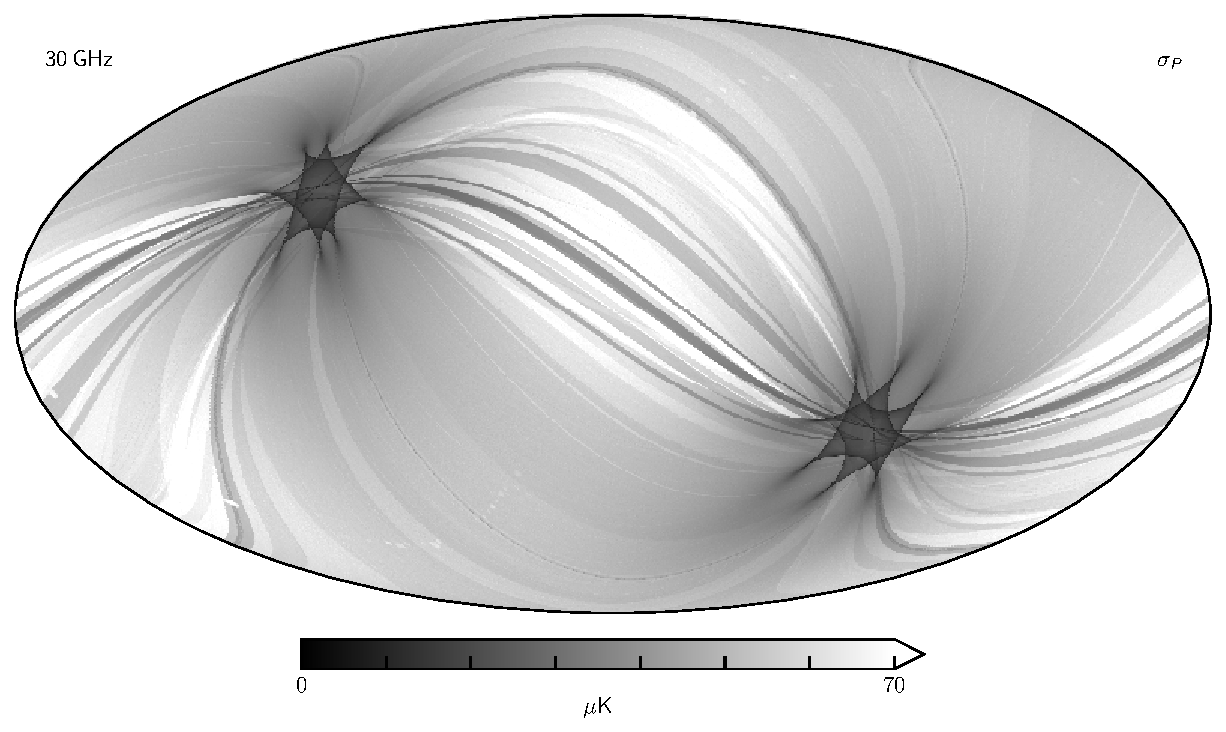
\includegraphics[width=0.35\textwidth]{figures/30GHz_sigmaP.pdf}\\
	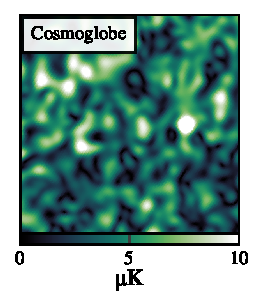
\includegraphics[width=0.212\textwidth]{figures/CG_square.pdf}
	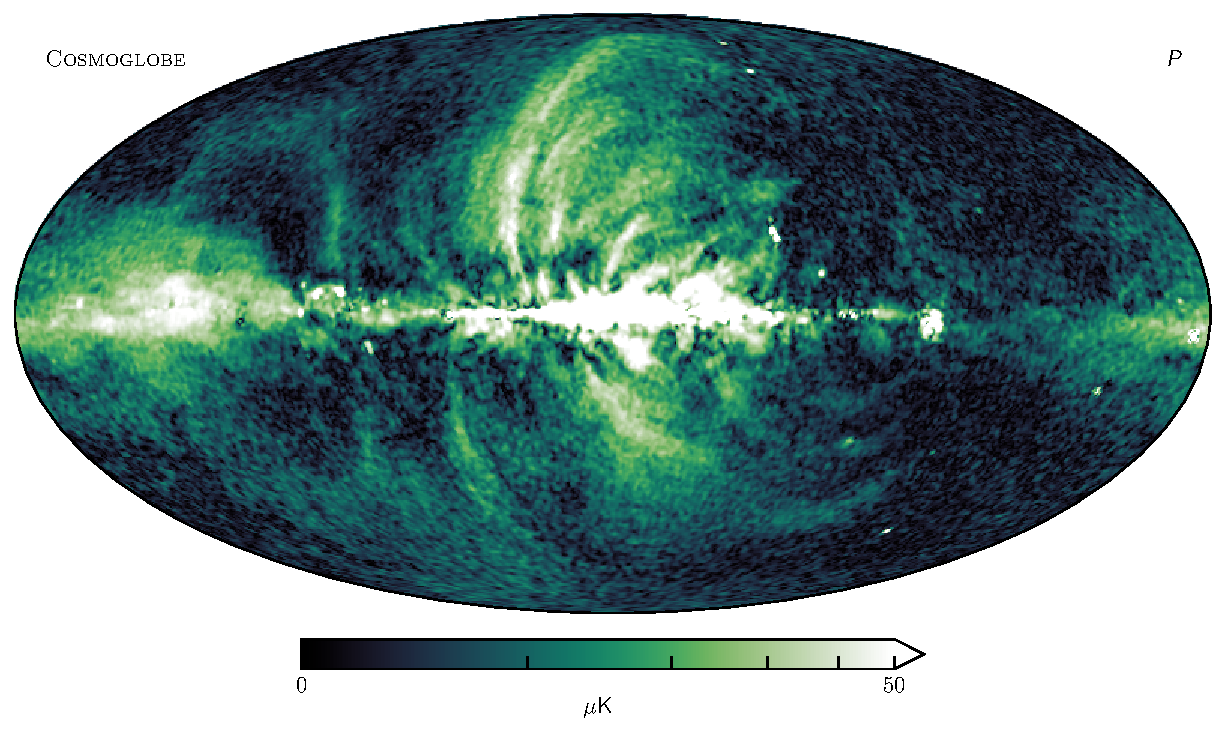
\includegraphics[width=0.35\textwidth]{figures/polint_CG.pdf}
	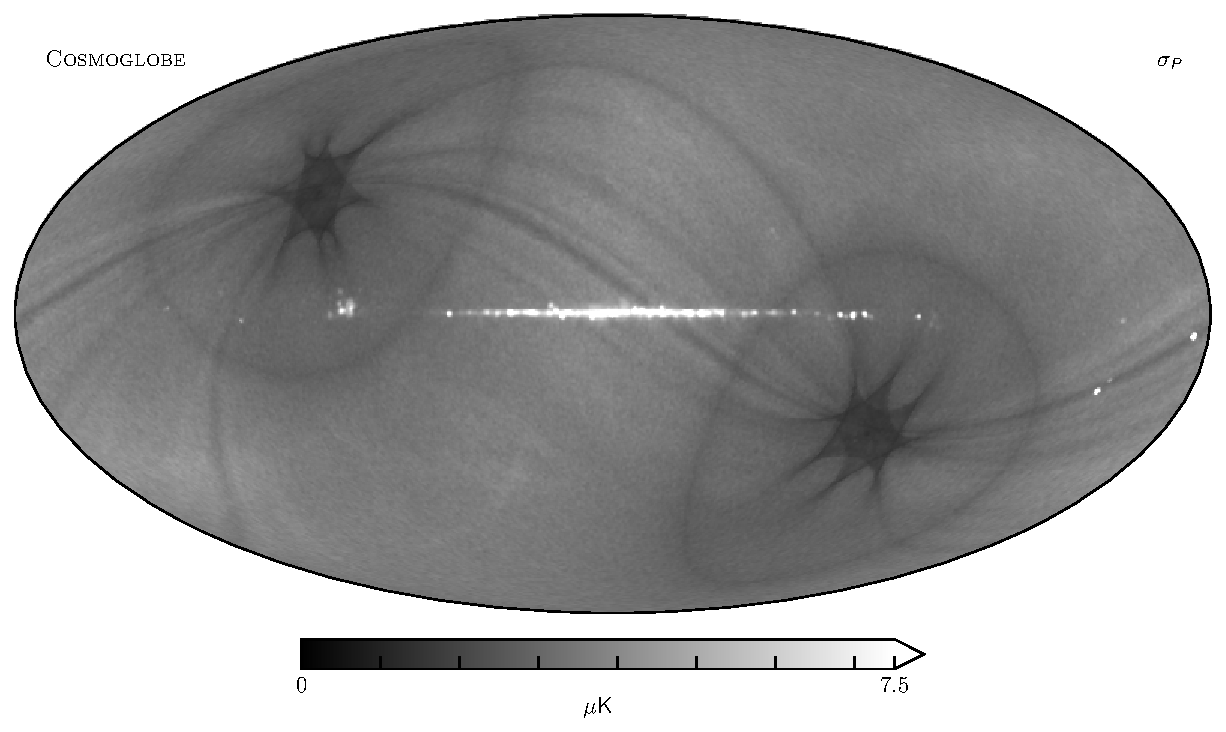
\includegraphics[width=0.35\textwidth]{figures/polint_CG_sigma.pdf}
	\caption{
		Polarized intensity and white noise levels of \textit{(top):} \WMAP\ \K-band, \textit{(middle):} \Planck\ 30\,GHz, and \textit{(bottom):} synchrotron amplitude from the \cosmoglobe\ Gibbs chain, all evaluated at 30\,GHz with a resolution of $72\arcm$. The leftmost column is a $10^\circ$ width square centered a low signal-to-noise regions highlighted by a red square in the top middle column's panels, the middle column shows the polarized total amplitude, $P$, and the rightmost column shows the rms noise for the frequency maps and the posterior standard deviation of the synchrotron amplitude.
		}
       \label{fig:synch_polint}
\end{figure*}


The data products used in this paper are the \WMAP\ and \Planck\ LFI maps, with most of the statistical weight coming from 23--33\,GHz, or the \WMAP\ \K\ and \Ka\ bands and LFI's 30\,GHz band. These frequencies are low enough that we can treat them as synchrotron tracers and hence ignore thermal dust and CMB emission, but not so low that we need to take into account effects like Faraday rotation, such as in S-PASS data \citep{krachmalnicoff2018,fuskeland:2019}. We describe the legacy data products and the data products from the \cosmoglobe\ \WMAP\ reanalysis in the following subsections.


\subsection{\WMAP\ and \Planck\ legacy products}
\label{sec:wmap_data}

\WMAP\ was a NASA-funded satellite mission that observed from August 2001 to August 2010, designed to characterize the microwave sky well enough to measure the primary CMB anisotropies across the full sky down to a resolution of 13\arcm\ FWHM. Using a differential scanning strategy inspired by \COBE/DMR,
\WMAP\ produced maps of the sky at 23 (\K), 33 (\Ka), 41 (\Q), 61 (\V), and 94\,GHz (\W) in both polarization and total intensity \citep{bennett2012}, with angular resolutions of 53\arcm\ at 23\,GHz to 13\arcm\ at 94\,\GHz. 
The maps are available on the LAMBDA website.\footnote{\url{https://lambda.gsfc.nasa.gov/product/wmap/dr5/m_products.html}} 

The \Planck\ Low Frequency Instrument (LFI) produced  30, 44, and 70 GHz maps in both intensity and polarization, while the High Frequency Instrument (HFI) produced 100, 143, 217, 353\,GHz maps in polarization and intensity, and 545 and 857\,GHz maps in intensity alone. The LFI data have somewhat lower white noise and higher angular resolutions (of 30\arcm, 20\arcm, and 13\arcm\ FWHM for 30, 44, and 70\,GHz) than \WMAP. In contrast to \WMAP, the LFI measurements used a single horn, and the \Planck\ scanning strategy followed rings closely aligned with ecliptic meridians. The \Planck\ legacy datasets, PR3 \citep{planck2016-l01} and PR4 \citep{planck2020-LVII}, are both publicly available on the \Planck\ Legacy Archive (PLA).\footnote{\url{https://pla.esac.esa.int/}}

\subsection{\Cosmoglobe\ products}
\label{sec:cosmoglobe_data}


A main goal of \Cosmoglobe\ is to perform joint end-to-end analyses on multiple data sets, preferably beginning from raw TOD. An important advantage of such end-to-end processing is that it offers a robust path to breaking internal degeneracies within and between different data sets, thereby in general reducing the magnitude of systematic effects. The analysis described by \citet{bp01} and \citet{watts2023_dr1} were performed on raw TOD, producing cosmological parameters using the Bayesian Gibbs sampler, \commanderthree\ \citep{bp03}. %The data products produced in this analysis accounts for the complex interactions between the instrument, the microwave sky, and its constituent components self-consistently. %\footnote{\url{https://www.cosmoglobe.uio.no/products/cosmoglobe-dr1.html}}
% Annoying error when there is hyphen in url...

In this framework, we produce a full sky model and set of instrumental parameters for each Gibbs sample, and the set of all such samples allows for a thorough characterization of the dependence of low-level instrumental parameters on the sky model. The sky model includes all relevant components in \WMAP\ and LFI's frequency range, specifically the CMB, synchrotron, thermal dust, free-free emission, anomalous microwave emission, and radio point sources, the first three of which we model as polarized in our sky model. The full products from this analysis and individual maps are available on the \cosmoglobe\ website.\footnote{\href{https://www.cosmoglobe.uio.no/products/cosmoglobe-dr1.html}{\texttt{https://www.cosmoglobe.uio.no/products/\newline cosmoglobe-dr1.html}}}

As described by \citet{watts2023_dr1}, \cosmoglobe\ DR1 includes 500 end-to-end Gibbs samples, and we perform our basic analysis on each of these samples individually, and then form posterior summary statistics from the full ensemble. This allows us to fully marginalize over the low-level systematic parameters, quantifying the extent to which instrumental processing propogates to the synchrotron spectral index determination.


\section{Polarized synchrotron amplitude}
\label{sec:pol_amp}

In this section, we give an overview of the polarized synchrotron amplitude properties. In Sec.~\ref{sec:pol_amp_map}, we focus on the map-based properties, and compare with independently processed results in Sec.~\ref{sec:comp_independent}. In Sec.~\ref{sec:powspec},  we evaluate the power spectrum of the polarized synchrotron map and compute the B-to-E ratio.

\subsection{Polarized amplitude maps}
\label{sec:pol_amp_map}


%When using external data for polarized foreground cleaning, the choices for high signal-to-noise full sky constraints are either \WMAP\ \K-band, \Planck\ LFI 30\,GHz, or models derived from combinations of these data, as in \cosmoglobe. From the perspective of pure statistical uncertainty, a combination of multiple independent datasets would yield component maps that are more sensitive than each individual component. However, unmodeled systematic uncertainties in the underlying datasets, left untreated, can induce map effects that can leak into astrophysics and cosmological constraints.
%As shown in \citet{watts2023_dr1}, a single sky model that all datasets are calibrated against improves the low-level instrumental processing, and allowing for degeneracies, such as transmission imbalance uncertainty in \WMAP\ and differential gain uncertainty in LFI, to be broken. Within the \cosmoglobe\ DR1 framework, the polarization maps from \WMAP\ and \Planck\ LFI are consistent with each other at the $10\,\mathrm{\mu K}$ level, consistent with the instrumental white noise of the datasets.

%The \cosmoglobe\ DR1 frequency maps are free from previously reported systematics, and are consistent between different frequencies and instruments. Therefore, a coherent model of polarized synchrotron emission can be made by combining the \WMAP\ and LFI frequency maps.

We start by comparing the polarized spectral amplitude (as defined by $P=\sqrt{Q^2+U^2}$) from the \cosmoglobe\ synchrotron map with the official \WMAP\ \K-band and \Planck\ 30\,GHz maps in the leftmost and middle columns of Fig.~\ref{fig:synch_polint}. The visible noise bias from plotting this positive definite quantity highlights the reduction in the noise level in the \cosmoglobe\ synchrotron map as compared to the \K-band and 30\,GHz maps. This is particularly visible in the leftmost column of Fig.~\ref{fig:synch_polint}, an inset of a high Galactic latitude, low signal region.
%The rightmost column shows the corresponding noise rms for each of the three maps for each pixel.


To quantify the noise improvement in the synchrotron maps over pure templates based on either \K-band or 30\,GHz maps, we compare the posterior standard deviation of the \cosmoglobe\ synchrotron map with the frequency maps' rms values. The posterior standard deviation maps are $\lesssim1\,\mathrm{\mu K}$ for \K-band, while temperature-to-polarization uncertainty in 30\,GHz contributes at the $2\,\mathrm{\mu K}$ level (see, e.g., \citealp{watts2023_dr1} and \citealp{bp10} for further details). An informative prior of $D_\ell=200\,\e^{-\ell(\ell+1)\sigma^2}\,\mathrm{\mu K^2}$, where $\sigma$ is the Gaussian width corresponding to a FWHM of 30\arcm, is applied during polarized synchrotron amplitude fitting, essentially downweighting low signal-to-noise fluctuations at angular scales $\lesssim30\arcm$, or $\ell\gtrsim360$ \citep{bp14}. Therefore, the rms noise contributions are relevant at roughly $N_\mathrm{side}=128$. To compare the \cosmoglobe\ white noise level with the \K-band and 30\,GHz white noise levels, we simulate realizations of the expected white noise smoothed to 72\arcm\ and scale the maps to 30\,GHz assuming $\beta_\mathrm s=-3.1$, consistent with the post-processed synchrotron map. We display these smoothed rms maps in the right column of Fig.~\ref{fig:synch_polint}.

At these resolutions, the mean rms for \K-band and 30\,GHz are $4.8\,\mathrm{\mu K}$ and $4.7\,\mathrm{\mu K}$ respectively, compared to the mean value of $3.4\,\mathrm{\mu K}$ for the \cosmoglobe\ DR1 synchrotron map; this is consistent with adding the scaled maps in quadrature.  While this may seem obvious on its face,  the combination of \WMAP\ \K-band and \Planck\ 30\,GHz is not straightforward due to instrumental effects that remain in the maps, notably poorly measured modes in \WMAP\ \citep{bennett2012,weiland:2018} and gain uncertainty in \Planck\ \citep{planck2016-l02}. These effects remain in the official \WMAPnine\ \citep{bennett2012} and \Planck\ PR3/PR4 \citep{planck2016-l02,planck2020-LVII} maps, making combination of these datasets non-ideal for Galactic science and cosmological analyses. However, the end-to-end \bp\ \citep{bp01} products effectively removed the gain uncertainty modes from the \Planck\ LFI maps, and the \cosmoglobe\ DR1 results \citep{watts2023_dr1} are free from the poorly measured modes. As shown in Fig.~46 of \citet{watts2023_dr1}, the \Planck\ 30\,GHz and the \WMAP\ \K-band are consistent with each other at the $10\,\mathrm{\mu K}$ level, indicating that the maps are consistent with each other down to the white noise level. This polarized synchrotron map, derived from consistent datasets, has a white noise level 29\,\% lower than both the \K-band map and the 30\,GHz map.%, with minimal systematic uncertainties in the posterior standard deviation. %Therefore, the synchrotron map derived from the \cosmoglobe\ DR1 Gibbs chain should be used for the characterization and removal of polarized synchrotron emission between 23--90\,GHz.



%The \WMAP\ \K-band data and LFI 30\,GHz data, as the highest signal-to-noise full-sky polarized maps of Galactic synchrotron emission, are the main contributors to our knowledge of the polarized amplitude. The slightly higher angular resolution 30\,GHz map has lower signal-to-noise than the \K-band data, but by combining the multi-resolution maps we are able to produce a clean map of the synchrotron emission evaluated at 30\,GHz with a FWHM of $1^\circ$.

%Each of these maps were produced with slightly different pipelines and datasets. The top row shows \Planck\ PR4 and \WMAPnine, and consists of entirely different datasets.\footnote{\textbf{Perhaps several samples of \WMAP-only would be useful to compare apples-to-apples, since these are all \commanderthree\ products.}} 

%The synchrotron solution is driven by the lowest frequency map, 30\,GHz and \K-band respectively, so any difference in the amplitude maps are due to differences in a combination of data processing, instrumental properties, and the microwave sky at 23\,GHz and 30\,GHz.


\begin{figure}
	%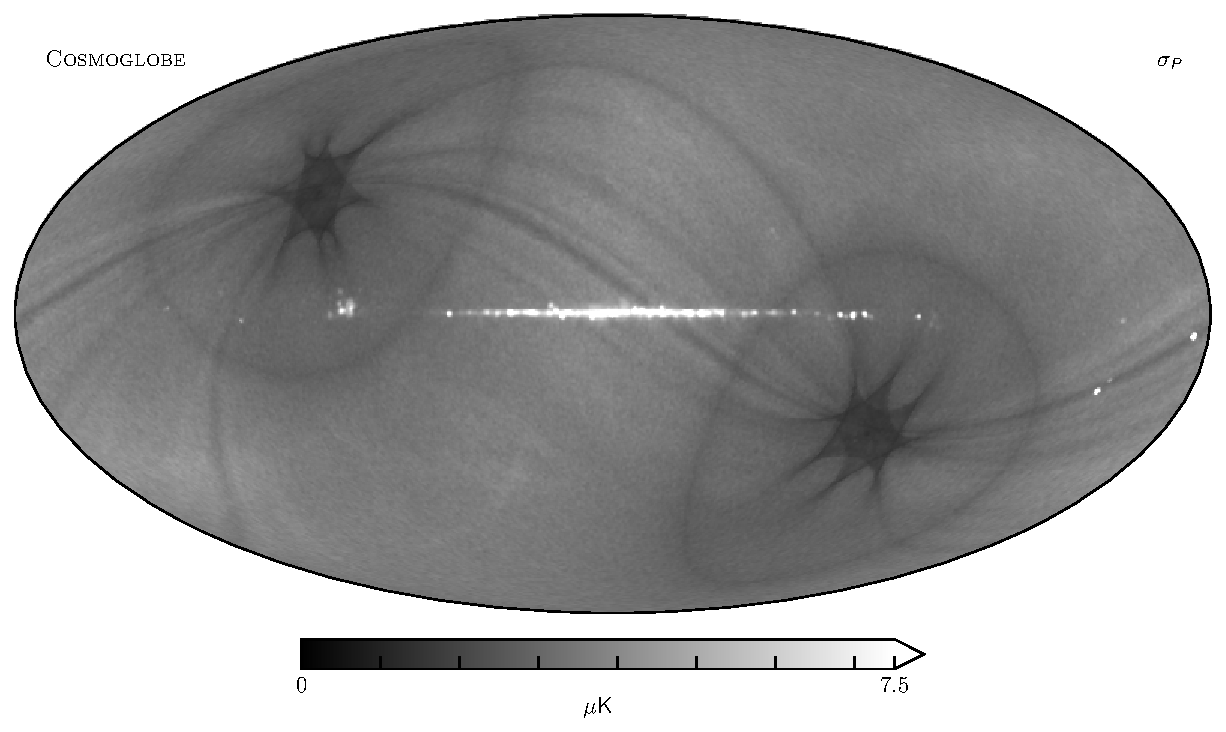
\includegraphics[width=0.45\textwidth]{figures/polint_CG_sigma.pdf}
	\centering
	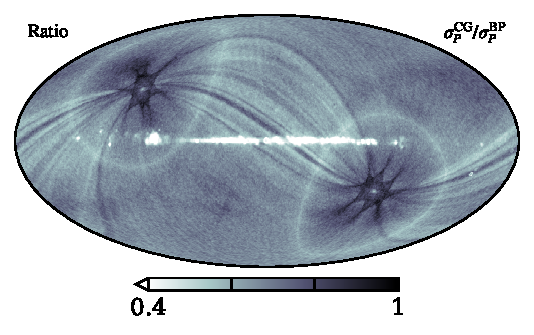
\includegraphics[width=0.45\textwidth]{figures/polint_sigma_ratio.pdf}
	\caption{
		%\textit{(Top:)} Posterior standard deviation of \cosmoglobe\ synchrotron polarization amplitude maps.
		\cosmoglobe\ posterior standard deviation divided by \bp\ posterior standard deviation.
		}
		\label{fig:rms_ratios}
\end{figure}

In Fig.~\ref{fig:rms_ratios} we plot the ratio between the \cosmoglobe\ and \bp\ \citep{bp01} synchrotron rms maps. Both these products are created using the \commanderthree\ pipeline and similar data selection, but \cosmoglobe\ benefits from additionally using the \K-band data. The \cosmoglobe\ synchrotron map has a mean posterior rms of $3.4\,\mathrm{\mu K}$, nearly a factor of two improvement over the \bp\ map.
%The rms map itself contains high signal-to-noise regions corresponding to the \WMAP\ circles about the ecliptic poles as well as the \Planck\ rings and multiple ecliptic polar crossings. The main clear astrophysical variation comes in the forms of a thin region about the Galactic plane and several low-latitude point sources. 
As expected, the regions with the lowest ratios correspond to the deep \WMAP\ observations and the Galactic plane, which benefit from the high signal-to-noise of the \K-band data. Regions with nearly identical rms include regions with the highest \Planck\ depth, such as the ecliptic poles, and regions less deeply observed by \WMAP, corresponding to planet crossings and artifacts from the processing mask. Notably, stripes corresponding the \Planck\ scan strategy also show improvement with respect to \bp. This is due to the interaction between the sky model and LFI's instrumental parameters --- with the high signal-to-noise \K-band data, the sky model becomes more stable, and LFI's relative gain solution becomes better determined.





%\subsection{Quantifying uncertainty}
%
%(Consider this Duncan's notes, because there are some details that are a bit fuzzy.)
%
%The \WMAP\ and \Planck\ rms maps are evaluated at pixelizations $N_\mathrm{side}=512$. If we simply downgrade maps, then the original noise per pixel scales as the area of the pixel, or $N_\mathrm{side,old}/N_\mathrm{side,new}$. For example, \K-band has an average rms of $91\,\mathrm{\mu K}$ at $N_\mathrm{side}=512$, while the same map at $N_\mathrm{side}=16$ has a white noise level of $\sim3\,\mathrm{\mu K}$, 32 times smaller.
%
%When we smooth a map, we are doing something quite similar to downgrading, except now we are correlating pixels as well, so the noise amplitude will decrease proportional to the area that the Gaussian is averaging over. The correlations make this a bit trickier to get effective rms maps that are truly diagonal, but we'll stick with it for now.
%
%The systematics are a bit different, since they don't actually average down with noise level, so for example, if you downgraded to $N_\mathrm{side}=8$, the poorly measured modes and the gain imbalance modes would not decrease. These are also a bit hard to see, so we smooth the maps an additional $2^\circ$.
%
%
%For simple template fitting, with
%\[
%	d_\nu = A\left(\frac{\nu}{\nu_0}\right)^\beta+n_\nu=AT_\nu+n_\nu,
%\]
%we have the simple result
%\[
%	\hat A=\frac{\sum_\nu T_\nu d_\nu/\sigma_\nu^2}{\sum_\nu T_\nu^2/\sigma_\nu^2},\qquad
%	\mathrm{var}(\hat A)=\frac1{\sum_\nu T_\nu^2/\sigma_\nu^2},
%\]
%so we would expect maps of the standard deviation of the synchrotron amplitude to look like inverse-weighted combinations of the data. This does seem to be the case, except we notice that the synchrotron map is evaluated at $N_\mathrm{side}=1024$ with a resolution of $40\arcm$, so the noise should actually be higher. Why isn't it?
%
%I think partly because a prior is imposed
%\[
%	\hat D_s(\ell)=200\,\e^{-\ell(\ell+1)\sigma^2(30\arcm)}\mathrm{\mu K^2},
%\]
%which basically kills off everything smaller than $30\arcm$, approximately $N_\mathrm{side}=128$. Perhaps this is the resolution we should limit ourselves to, since these are the only scales that really contribute?
%
%I think that is fair, since it's also roughly where the white noise starts to dominate, $\ell=100$.
%
%As stated in \citet{bp14}, we use scale-dependent priors in component separation so that the prior will play a negligible role in signal-dominated regions, but play a stronger role in noise-dominated regions.


\subsection{Comparison with independent datasets}
\label{sec:comp_independent}

\begin{figure*}
	\begin{center}
	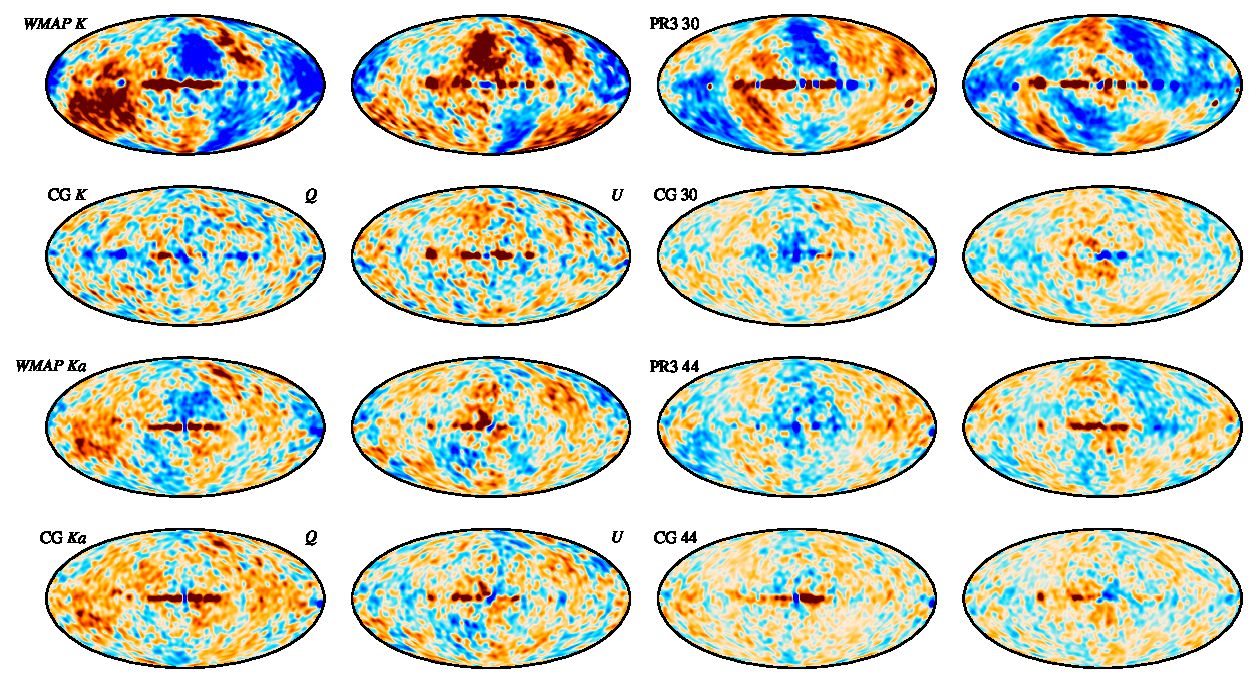
\includegraphics[width=\textwidth]{figures/CG_DR1_residuals.pdf}
        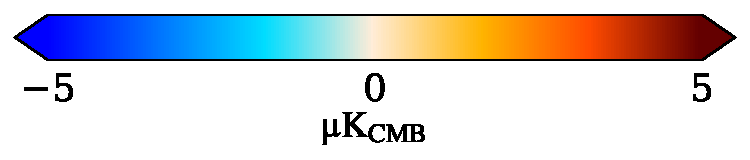
\includegraphics[width=0.25\textwidth]{figures/cbar_5uK.pdf}
	\end{center}
	\caption{Frequency map minus sky model residuals with respect to the \cosmoglobe\ DR1 sky model evaluated at $5^\circ$. \cosmoglobe\ maps are labeled CG, \Planck\ 2018 maps are labeled PR3, and the legacy \WMAPnine\ maps are labeled \WMAP. Each of the \WMAPnine, \Planck\ PR3, and \cosmoglobe\ maps have had the \cosmoglobe\ DR1 sky model evaluated at their respective bandpass and resolution subtracted. 
	}
	\label{fig:cg_residuals}
\end{figure*}

Next, we compare the \cosmoglobe\ polarized synchrotron map with the frequency maps produced in the main DR1 chain, paying special attention to maps with the highest polarized synchrotron signal-to-noise ratio; \K, \Ka, 30\,GHz, and 44\,GHz.
Using the polarized synchrotron model generated in the main \cosmoglobe\ DR1 chain, we evaluate the synchrotron emission at each frequency and subtract this from frequency maps produced by various different processing pipelines. We evaluate the \cosmoglobe\ sky model using the \texttt{cosmoglobe} Python package to evaluate the sky model using the full bandpass information of each instrument.\footnote{\url{https://cosmoglobe.readthedocs.io/en/latest/tutorials/skymodel.html}} %Visual inspection of the data with the sky model subtracted and smoothed to a common $5^\circ$ Gaussian beam provides a robust check on the quality of the model and the underlying data.

%These maps should agree by virtue of being produced in the same analysis framework. We compare with the \WMAPnine\ and PR3 maps. Of these, the \WMAPnine\ results can be considered the most independent, as the results were produced with no sky model assumptions, and were produced before the \Planck\ polarized maps were publicly available, thus making the analysis completely unbiased. The PR3 maps should also be independent of the \WMAPnine\ results, although the \WMAPnine\ results were available during PR3 production, so this analysis cannot be truly considered blinded to existing \WMAP\ data.
%The PR4 analysis was performed using both the LFI and HFI dataset in a joint processing framework, conceptually similar to the framework in \cosmoglobe\ DR1. Since we are highlighting the differences between joint processing and independent processing frameworks, we leave out PR4 in this specific comparison.

The first and third rows of Fig.~\ref{fig:cg_residuals} show the \WMAPnine\ and PR3 residuals with respect to the \cosmoglobe\ sky model in second and fourth rows. These residuals match previously-documented observational effects in both experiments. In particular, the \WMAP\ maps show artifacts of the poorly-measured modes due to transmission imbalance in the differential horns \citep{jarosik2007,bennett2012}, while the PR3  differences are mostly  due to relative gain errors \citep{planck2016-l02,planck2020-LVII}.
In contrast, the synchrotron model matches the \cosmoglobe\ DR1 frequency maps within $5\,\mathrm{\mu K}$ across the sky, with few observational artifacts.

Most of the residuals are associated with the Galactic plane and diffuse structures uncorrelated with the \WMAP\ and \Planck\ observation strategies. The positive excess in the \Ka\ Stokes $Q$ map could be due to unmitigated data processing artifacts. While a similar large-scale excess can also be seen in the LFI 30 and 44\,GHz Stokes $Q$ maps, the signature strongly resembles the bandpass correction in \WMAP\ \K-band, suggesting incomplete treatment of bandpasses could be contributing to this large-scale signal.
The LFI residuals, while much improved, still show trace residuals, especially near the Galactic center, that are somewhat correlated with the gain correction templates, but not at a level that high Galactic latitude features can be identified. 

As the scale of instrumental residuals have been reduced to below the white noise level for each of the synchrotron-dominated full-sky polarization maps, we are now able to associate the residuals with potential modifications to the sky model. Specifically, the \cosmoglobe\ DR1 processing sampled a spatially constant $\beta_\mathrm s$ with a final mean of $\beta_\mathrm s=-3.15$. In Sec.~\ref{sec:specvar}, we analyze these maps allowing for spatial dependence in the polarized synchrotron spectral index to determine the extent to which true on-sky variation can be determined based on these maps.


\subsection{Power spectra}
\label{sec:powspec}

% Add a bit more?

Next, we consider the angular power spectrum of polarized synchrotron emission. To estimate the power spectra without a noise bias, we perform a \commanderthree\ run using half-mission splits with odd-numbered scans and even-numbered scans being analyzed in runs labeled HM1 and HM2, analogous to the \Planck\ ``half-mission'' splits. Each of these chains were performed using the same data as in the main \cosmoglobe\ chain, with 200 samples each.\footnote{These products can be found at \url{cosmoglobe.uio.no}.}
The highest quality of similar half-mission splits that are publicly available are from the \Planck\ PR3 analysis, as discussed in \citet{planck2016-l04}. We therefore compute power spectra from the PR3 results and compare them directly with the \cosmoglobe\ HM splits.


%We perform cross-spectra to avoid an additive noise bias.

We perform power spectrum estimation using \texttt{NaMaster} \citep{namaster} with the \Planck\ 2018\ common polarization mask with $f_\mathrm{sky}=0.78$ and $1^\circ$ apodization.
To quantify the uncertainty, we take the cross spectrum for each pair of Gibbs samples from HM1 and HM2 respectively, and report the 68\,\% confidence intervals on this posterior. The power spectra are displayed in Fig.~\ref{fig:spectra}, and the standard deviation is computed using the within-bin variance of each bin, with the posterior standard deviation of the Gibbs chain added in quadrature for the \cosmoglobe\ spectra.
Other than the very lowest and very highest multipole bins, there is good per-multipole agreement between both the PR3 and \cosmoglobe\ DR1 spectra. For comparison, we plot the $E$-mode power spectrum predicted by the \Planck\ 2018 cosmological parameters.

Following \citet{planck2016-l04}, we perform power law fits to the power spectra of the form $\mathcal D_\ell^\mathrm{EE/BB}=A_s^{\mathrm{EE/BB}}(\ell/80)^\alpha$, using multipoles $\ell\in[2,140]$. The 68\,\% confidence intervals for each quantity, including the $A_s^\mathrm{BB}/A_s^\mathrm{EE}$ ratio, are reported in Table~\ref{tab:synch_powspec}. The primary differences between the fits to the two datasets are $\sim2~\sigma$ discrepancies in the $A_s^\mathrm{BB}$ and $\alpha_s^\mathrm{EE}$ fits, while all others are consistent within $\simeq0.5~\sigma$. The primary drivers of these differences are lower $\mathcal D_\ell^\mathrm{BB}$ and higher $\mathcal D_\ell^\mathrm{EE}$ in the lowest bins.

A question of special interest is the ratio of synchrotron $B$-mode to $E$-mode power, which has been consistently noted to be less than one \citep{page2007,planck2014-a12,planck2016-l04,krachmalnicoff2018,QUIJOTE_IV,eimer2023}. The physical mechanism for this has been discussed in the context of Galactic magnetic fields and polarized thermal dust (e.g., \citealp{kandel2017}, \citealp{so_galci}, \citealp{vacher2023}), but similar mechanisms are likely to be in play for synchrotron polarization. In Table~\ref{tab:synch_powspec}, we find a value of $A_s^\mathrm{BB}/A_s^\mathrm{EE}$ of 0.40 for the \cosmoglobe\ splits and 0.46 for PR3. In this respect, we note that our value of $A_s^\mathrm{BB}/A_s^\mathrm{EE}$ for \Planck\ 2018 is higher than that reported by \citet{planck2016-l04} of 0.34, despite using nearly identical methodology. The origin of this discrepancy is not yet understood, but it must necessarily be associated with details in  the power spectrum estimation algorithm. %The ratio we determined for the PR3 split is lower than the reported value of 0.34 in \citet{planck2016-l04}, using a nearly identical methodology. Despite the discrepancies between the values in this paper and \citet{planck2016-l04}, it is clear that the \cosmoglobe\ DR1 ratio is lower than that of \Planck\ PR3.

\begin{figure}
        \centering
	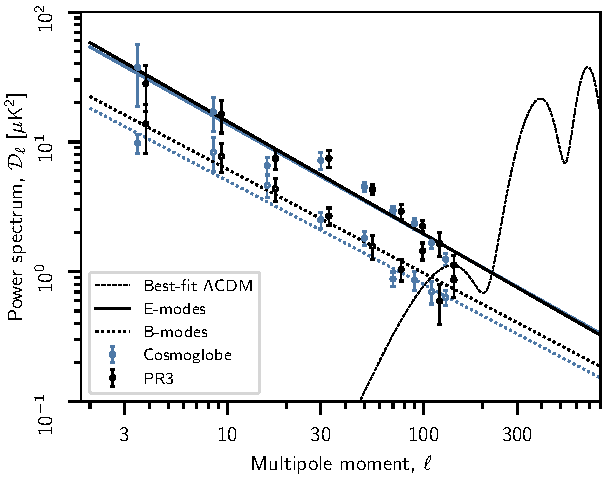
\includegraphics[width=\linewidth]{figures/cls_synch_ratio.pdf}
        \caption{
		Half-mission cross spectra for polarized synchrotron emission as evaluated for \Planck\ PR3 (black) and \cosmoglobe\ DR1 (blue). Filled circles correspond to $E$-modes, while empty circles correspond to $B$-modes. The thick solid and dashed lines are the best-fit $E$- and $B$-mode power law fits to synchrotron, and the thin black line is the $\Lambda$CDM prediction for $E$-modes.
        }
        \label{fig:spectra}
\end{figure}


\begin{table}
\newdimen\tblskip \tblskip=5pt
	\caption{Best-fit power law parameters to the synchrotron estimates evaluated at 30\,GHz, using half-mission cross-spectra evaluated with \texttt{NaMaster}.}
\label{tab:synch_powspec}
\vskip -5mm
\footnotesize
\setbox\tablebox=\vbox{
 \newdimen\digitwidth
 \setbox0=\hbox{\rm 0}
 \digitwidth=\wd0
 \catcode`*=\active
 \def*{\kern\digitwidth}
%
  \newdimen\dpwidth
  \setbox0=\hbox{.}
  \dpwidth=\wd0
  \catcode`!=\active
  \def!{\kern\dpwidth}
%
  \halign{\hbox to 1.8cm{#\leaderfil}\tabskip 2em&
    \hfil$#$\hfil \tabskip 2em&
    \hfil$#$\hfil \tabskip 0em\cr
\noalign{\doubleline}
	\omit\hfil \hfil& \mathrm{PR3} & \cosmoglobe\cr
\noalign{\vskip 3pt\hrule\vskip 5pt}
	$A_s^\mathrm{EE}$ [$\mathrm{\mu K^2}$]                & \phantom{-}2.39 \pm 0.07 & \phantom{-}2.35 \pm 0.05 \cr
	$A_s^\mathrm{BB}$ [$\mathrm{\mu K^2}$]                & \phantom{-}1.09 \pm 0.06 & \phantom{-}0.94 \pm 0.04 \cr
	$A_s^\mathrm{BB}/A_s^\mathrm{EE}$ & \phantom{-}0.46 \pm 0.03 & \phantom{-}0.40 \pm 0.02 \cr
	$\alpha_s^\mathrm{EE}$            & -0.81 \pm 0.02 & -0.87 \pm 0.02 \cr
	$\alpha_s^\mathrm{BB}$            & -0.80 \pm 0.03 & -0.81 \pm 0.03 \cr
%
\noalign{\vskip 5pt\hrule\vskip 5pt}}}
\endPlancktablewide
\end{table}



\section{Polarized synchrotron spectral indices}

\label{sec:specvar}

The determination of polarized synchrotron spectral index variation across the sky has been studied in detail using several different data combinations. Although the small-scale details vary, nearly every analysis has found $\beta_\mathrm s\simeq2.8$ in the Galactic plane and $\beta_\mathrm s\sim-3.3$ in high Galactic latitudes \citep{fuskeland2014,krachmalnicoff2018,fuskeland:2019,weiland:2022}, with the exception of QUIJOTE \citep{QUIJOTE_IV,QUIJOTE_VIII}, who find a slightly flatter spectral index along the Galactic plane.
Both \citet{fuskeland2014} and \citet{weiland:2022} report oscillations with Galactic longitude close to the Galactic plane, but high-latitude regions variations are more difficult to determine, and tend to depend on the specific dataset chosen and the analysis method chosen.

A fundamental challenge in spectral index estimation is due to the fact that every difference between two channels can be associated with a spectral index variation if not accounted for fully. Therefore, it is necessary to not only make sure that results are robust towards data selection, but also to ensure that differences between results are not due to instrumental effects.


While the \cosmoglobe\ pipeline produces samples of polarized synchrotron emission, the spatial variation of the spectral index is poorly determined within the Gibbs chain. To mitigate the poor Monte Carlo Markov Chain (MCMC) convergence of the spectral indices, the \cosmoglobe\ DR1 sampled the spectral index from a prior distribution, $\beta_\mathrm s\sim\mathcal N(-3.15, 0.05)$. Improvements within the \commanderthree\ framework will require more high signal-to-noise data.

In order to test for and mitigate potential instrumental effects, we perform two analyses, a temperature-temperature (T-T) plot analysis in Sect.~\ref{sec:tt_plot} and a Gibbs sampling analysis using \commanderone\ in Sect.~\ref{sec:comm1}. Section~\ref{sec:tt_plot} focuses on pairs of channels to better isolate potential unmodeled systematic effects, while Sect.~\ref{sec:comm1} uses all \WMAP\ and LFI channels plus \Planck\ 353\,GHz to maximize the joint statistical weight of all available data.

\subsection{T-T plot analysis}
\label{sec:tt_plot}

The T-T plot analysis can be used for pairs of datasets in a model-independent way, allowing for us to probe the difference between different datasets without making strong assumptions on the underlying physical model. This method can also easily be adapted to probe the dependence on polarization angle. This can be used to determine both the orientation dependence of $\beta_\mathrm s$, as well as identify the magnitude of unmodeled instrumental effects, such as beam asymmetries, as discussed in \citet{wehus:2013}.


\begin{figure}
        \centering
        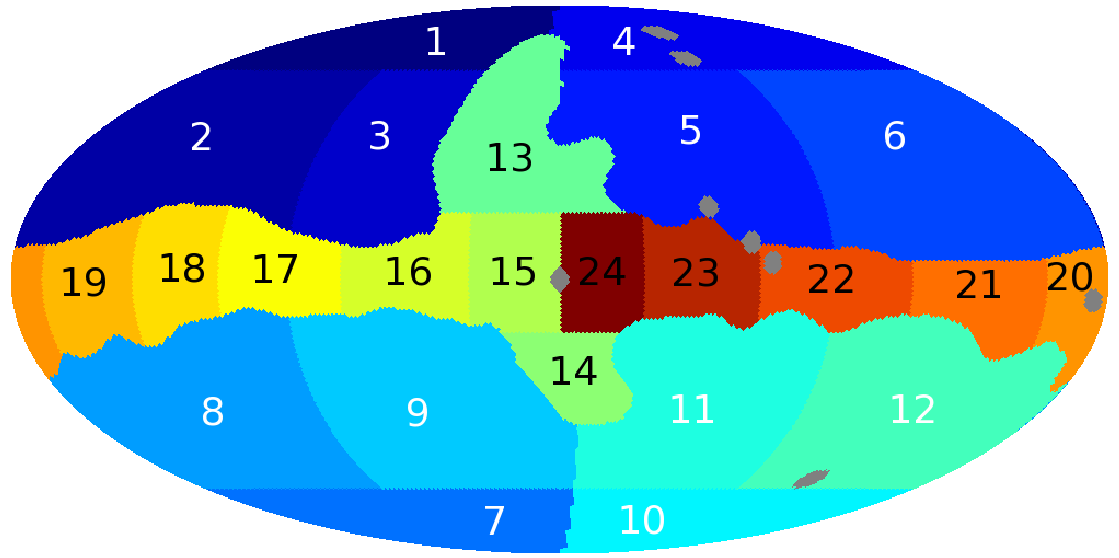
\includegraphics[width=\linewidth]{figures/utnymaske_tall_converted.pdf}
        \caption{Spectral index regions as defined in \citet{fuskeland2014}. The most prominent point sources are masked out and shown in grey circular areas.
        }
        \label{fig:regions}
\end{figure}

\subsubsection{Method}
\label{sec:tt_plot_method}

Following \citet{fuskeland2014} and \citet{fuskeland:2019}, we apply linear regression via the T-T plot method, in which spectral indices can be estimated over extended regions with approximately constant spectral indices. Here we use the regions labeled in Fig.~\ref{fig:regions}. In this approach, our data model for two frequencies is
\begin{equation}
	\boldsymbol m_\nu = \boldsymbol m_{\nu_0}\left(\frac\nu{\nu_0}\right)^\beta+c_\nu+\boldsymbol n_\nu ,
\end{equation}
where $\boldsymbol m_\nu$ is a spatially varying amplitude map at frequency $\nu$, $\nu_0$ is the reference frequency, $\beta$ the power law between the two frequencies, $c_\nu$ the spatially constant offset per band, and $\boldsymbol n_\nu$ the noise.  In the case of noiseless data with no offset, the spectral index may be estimated using a simple ratio,
\begin{equation}
	\frac{m_{\nu_1,p}}{m_{\nu_2,p}}
	=\left(\frac{\nu_1}{\nu_2}\right)^{\beta_{s,p}}
	\Rightarrow
	\beta_{s,p}=\frac{\ln(m_{\nu_1,p}/m_{\nu_2,p})}{\ln(\nu_1/\nu_2)}.
\end{equation}
In the case where one map is much noisier than the other, the standard T-T plot method involves performing  a linear regression $\boldsymbol m_{\nu_1}=a\boldsymbol m_{\nu_2}+b$, and associates $\beta_s$ with $\ln a/\ln(\nu_1/\nu_2)$. More care must be taken when the noise amplitudes in both maps are comparable to each other, so we adopt the effective variance method of \citet{orear1982} as implemented by \citet{fuskeland2014}.

For the T-T plot  analysis, we focus exclusively on bands between 23 and 33\,GHz. As in \citet{fuskeland2014}, we use the \WMAP\ \K\ and \Ka\ band Stokes $Q$ and $U$ parameter maps at $23$\,GHz and $33$\,GHz. The respective effective frequencies used are $22.45$\,GHz and $32.64$\,GHz. The maps originally at a \healpix\footnote{\url{http://healpix.sourceforge.net}} pixelization of $N_\textrm{side}=512$ are downgraded to $N_\textrm{side}=64$ and smoothed to a common resolution of $1^\circ$ FWHM.
The \Planck\ data products used are the $30$\,GHz Stokes $Q$ and $U$ maps, with an effective frequency of $28.4$\,GHz. Both the \bp\ and \cosmoglobe\ products are natively at $N_\textrm{side}=512$, while for the \Planck\ PR4, it is 1024.



\begin{figure}
        \centering
	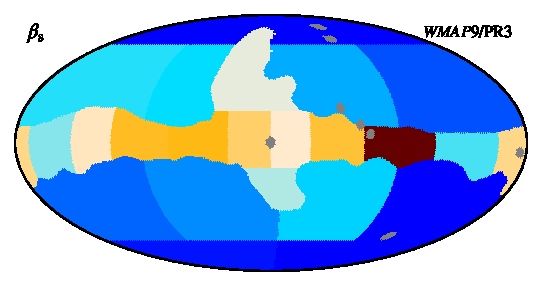
\includegraphics{figures/TT_map_W9PR3_K30.pdf}\vspace{-0.25cm}\\
	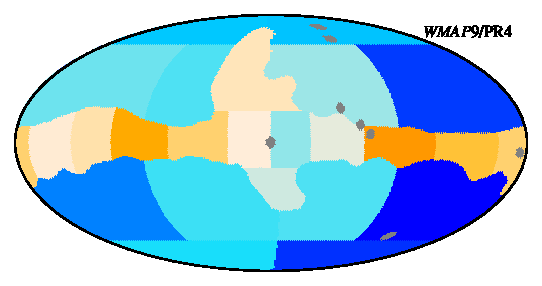
\includegraphics{figures/TT_map_W9PR4_K30.pdf}\vspace{-0.25cm}\\
	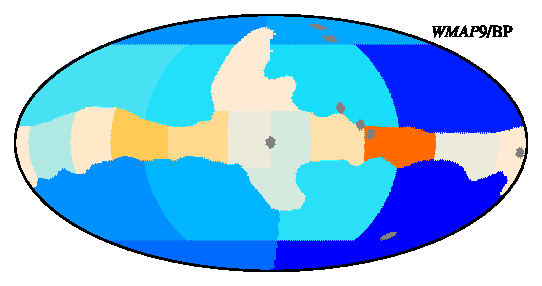
\includegraphics{figures/TT_map_W9BP_K30.pdf}\vspace{-0.25cm}\\
	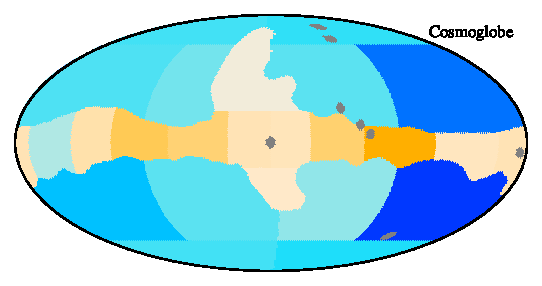
\includegraphics{figures/TT_map_CG_K30.pdf}\vspace{-0.25cm}\\
	\hspace{0.25cm}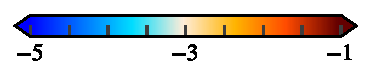
\includegraphics{figures/cbar_beta_wide.pdf}
	\caption{Spatial variation of the synchrotron spectral index, computed using T-T plot between the (from top to bottom) \WMAPnine\ \K-band and \Planck\ PR3 30\,GHz, \WMAPnine\ \K-band and \Planck\ PR4 30\,GHz, \WMAPnine\ \K-band and \BP\ 30\,GHz, and \Cosmoglobe\ \K-band and \Cosmoglobe\ 30\,GHz. The spectral index is inverse variance weighted over rotation angle, and in the \Cosmoglobe\ case also samples.}
        \label{fig:TT_beta_maps}
\end{figure}

As in \citet{fuskeland:2019}, a systematic uncertainty that takes into account the variation of $\beta$ over rotation angle, $[ \max(\beta_\alpha) - \min(\beta_\alpha) ] /2$, is added in quadrature to the statistical uncertainty.
The uncertainty of the spectral indices is calculated as the minimum of the uncertainties in each rotation angle and region. 
For the \Cosmoglobe\ analyses we have a whole suite of maps represented by the individual samples instead of just one mean map. Here the standard deviation of the spectral indices of the samples is also added in quadrature to represent an additional systematic uncertainty. This enables us to have a better propagation of uncertainties from the maps to the final spectral indices.

\begin{figure}
        \centering
        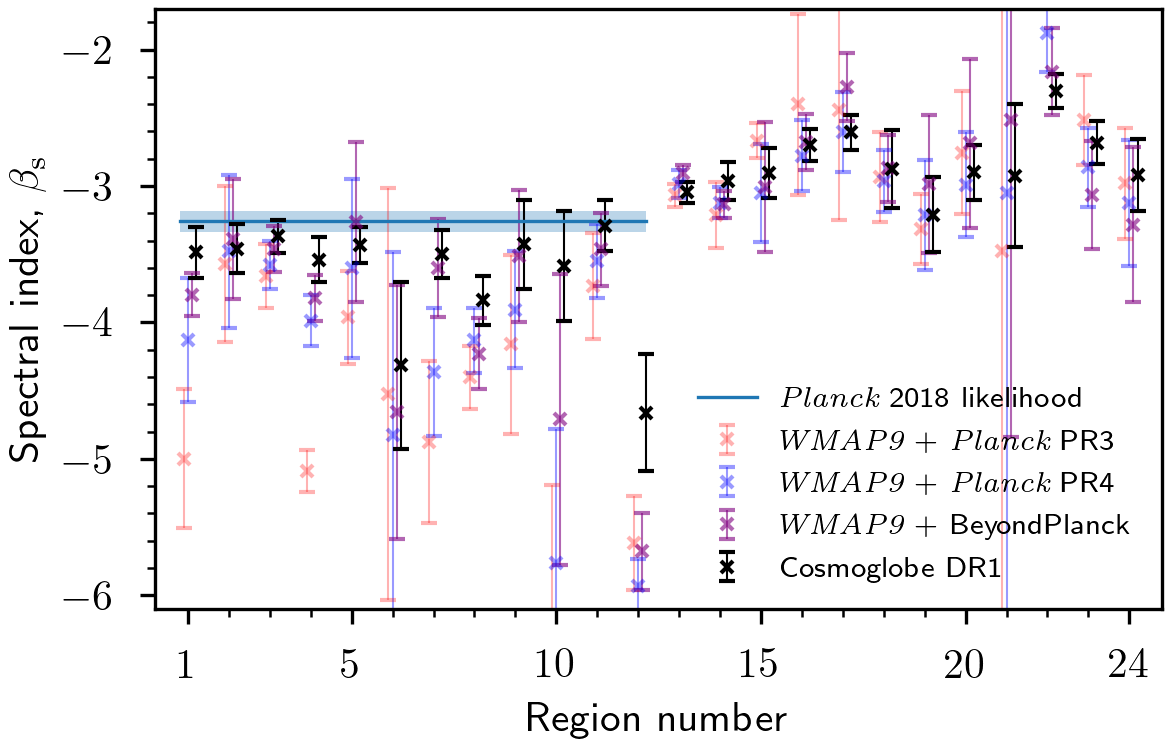
\includegraphics[width=\linewidth]{figures/cos30_region_beta_cosmoglobe_vs_wmap_all.png}
        \caption{Synchrotron spectral index as a function of region number, computed using T-T plot between the \WMAPnine\ \K-band and \Planck\ PR3 30\,GHz (red), \WMAPnine\ \K-band and \Planck\ DR4 30\,GHz (blue), \WMAPnine\ \K-band and \BP\ 30\,GHz (purple), and \Cosmoglobe\ \K-band and \Cosmoglobe\ 30\,GHz (black). The spectral index is inverse variance weighted over rotation angles, and samples. The horizontal line in the high latitude regions corresponds to the estimated spectral index values from the \Planck\ 2018 likelihood analysis \citep{planck2016-l05}. }
        \label{fig:cos30_beta_region}
\end{figure}

\subsubsection{Results}
\label{sec:tt_plot_results}

We start by looking at the results from the T-T plot method applied to the \K-band and 30\,GHz maps. We apply the method to the 24 regions to see the spatial variation of the polarized synchrotron spectral index. The top three maps in Fig. \ref{fig:TT_beta_maps} show the T-T plot results using \WMAPnine\ \K-band and three incarnations of the \Planck\ 30\,GHz maps; PR3, PR4, and \bp. The bottom map shows the results using the improved maps from the \cosmoglobe\ analysis, \K-band and 30\,GHz. The spectral indices are inverse variance weighted over rotation angle, and in the \cosmoglobe\ case also over posterior samples. Some of the brightest point sources have been masked out using grey. We see an overall narrowing in the range of spectral spectral indices, from regions with extreme values in the top map represented by dark red and blue values, with colors gradually fading in the lower figures. The range in the plot is quite wide for spectral indices, and goes from $-5$ to $-1$. This improvement in the value of the spectral index is especially prominent in the high Galactic regions, as well as region  number 22 along the Galactic plane.  Using the \cosmoglobe\ DR1 data, we find a full-sky inverse variance weighted mean of the spectral index, $\beta_{\mathrm{s}}=-3.07\pm0.07$ while the mean of the high latitude regions 1--14 is $-3.31\pm0.07$.

The same results are also shown in Fig. \ref{fig:cos30_beta_region}, with the spectral indices plotted as a function of region number. The different datasets are shown in different colors, and with the same order as the four maps in Fig.~\ref{fig:TT_beta_maps}. Here we have also included one sigma uncertainties as errorbars as described in Sect. \ref{sec:tt_plot_method}. The magnitude of the error bars are set by the reported white noise level in each dataset except for the \cosmoglobe, which also takes into account systematic uncertainties. We also plot the estimated spectral index range for high Galactic regions, in our case represented by regions 1--12, as forecasted by the likelihood analysis in Figure 22 of \citet{planck2016-l05}. We see with each iteration of the data processing, the region estimates draw closer to this line.
For a more detailed study of each of the regions, we refer the reader to Appendix \ref{sec:appendix}, where we have shown the corresponding T-T scatterplots (Fig.~\ref{fig:cos30_beta_bigscatter}) and the spectral index as a function of rotation angle (Fig.~\ref{fig:cos30_beta_bigalpha}) for all 24 regions.

As a second part of this T-T plot analysis we apply the method on \K-band and \Ka-band maps. For the \wmap\ data, this analysis was already performed in  \citet{fuskeland2014}, so here we only present results using the new \cosmoglobe\ data. First, as a consistency check, in Fig.~\ref{fig:cos30_xyplot} we plot the spectral indices for all 24 regions in the form of \cosmoglobe\ \K/30\,GHz versus \cosmoglobe\ \K/\Ka. We see that for the regions in the north and south Galactic spurs, and along the Galactic plane (regions 13-24), there is a good agreement between the spectral indices obtained by the two pairs of datasets. Regions 1--12, all of which are high-latitude regions with low signal-to-noise, are all consistent with the two data combinations. The most prominent outliers, regions 6 and 12, are the regions with the lowest signal-to-noise ratio, and hence most prone to unmodeled effects and noise fluctuations.

In Fig.~\ref{fig:beta_map} the value of the spectral indices is shown for the 24 regions. We see here that the colors are even fainter than the \cosmoglobe\ \K-band versus 30\,GHz values (the bottom figure in Fig.~\ref{fig:TT_beta_maps}), meaning there are fewer outliers with respect to a standard value in the range around $-3$. This is especially visible in the regions with lowest signal to noise, like regions 6, 8 and 12, at high latitude. Taking the inverse variance weighted mean of the spectral indices of all 24 regions, we get $\beta_{\mathrm{s}}=-2.95\pm0.07$, while for the high latitude regions 1--14 we get $-3.20\pm0.10$.


\begin{figure}
        \centering
        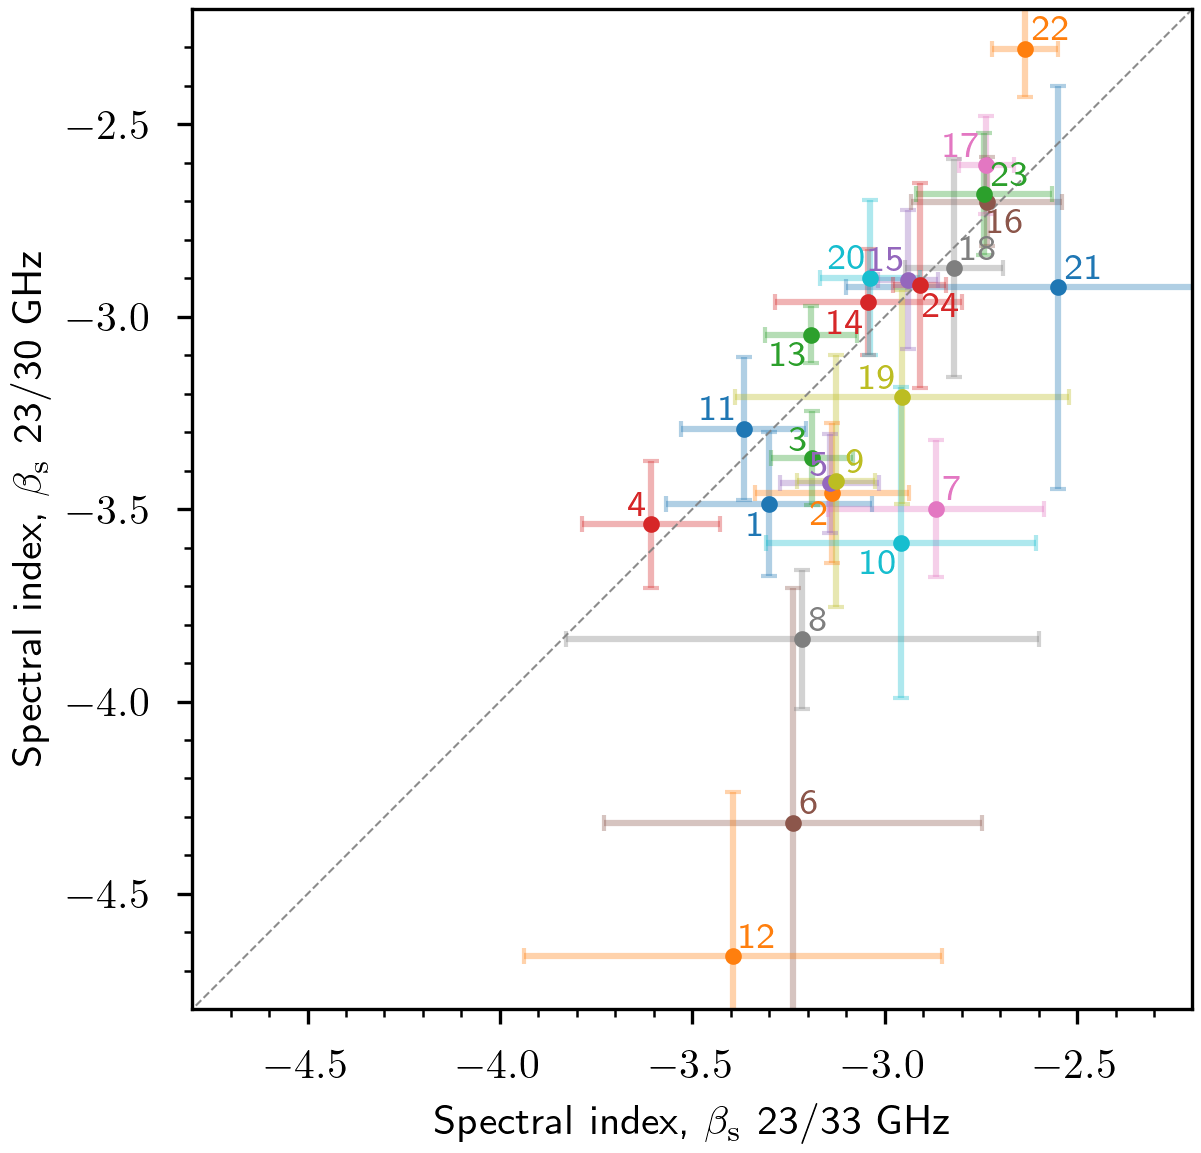
\includegraphics[width=\linewidth]{figures/xy_regions.png}
        \caption{
Synchrotron spectral index computed using T-T plot with the \Cosmoglobe\ DR1 \K-band and 30\,GHz data versus \Cosmoglobe\ DR1 \K-band and \Ka-band data for the 24 regions.}
        \label{fig:cos30_xyplot}
\end{figure}


\begin{figure}
	\centering
	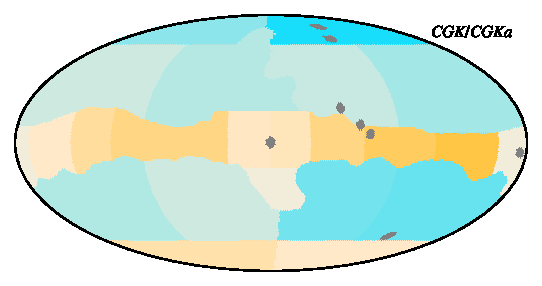
\includegraphics{figures/TT_map_CG_KKa.pdf}\vspace{-0.25cm}\\
	\hspace{0.25cm}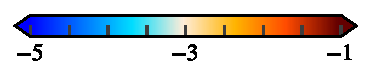
\includegraphics{figures/cbar_beta_wide.pdf}
	\caption{Spatial variation of the synchrotron spectral index, computed using T-T plot between the \Cosmoglobe\ DR1 \K- and \Ka-band. The spectral index is inverse variance weighted over rotation angle and samples.}
        \label{fig:beta_map}
\end{figure}


%\begin{figure*}
%	\centering
%	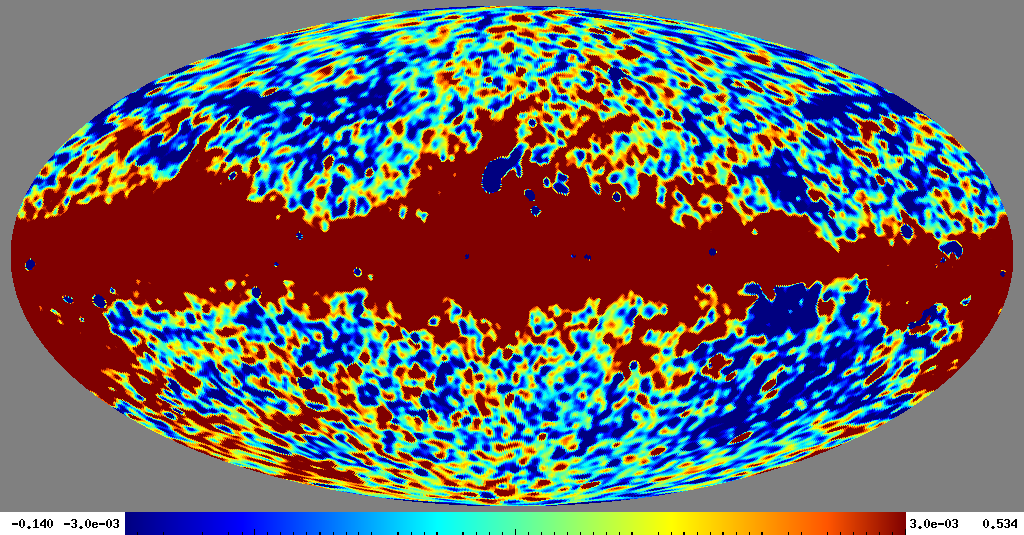
\includegraphics[width=0.40\linewidth]{figures/res_K_spdust.png}
%        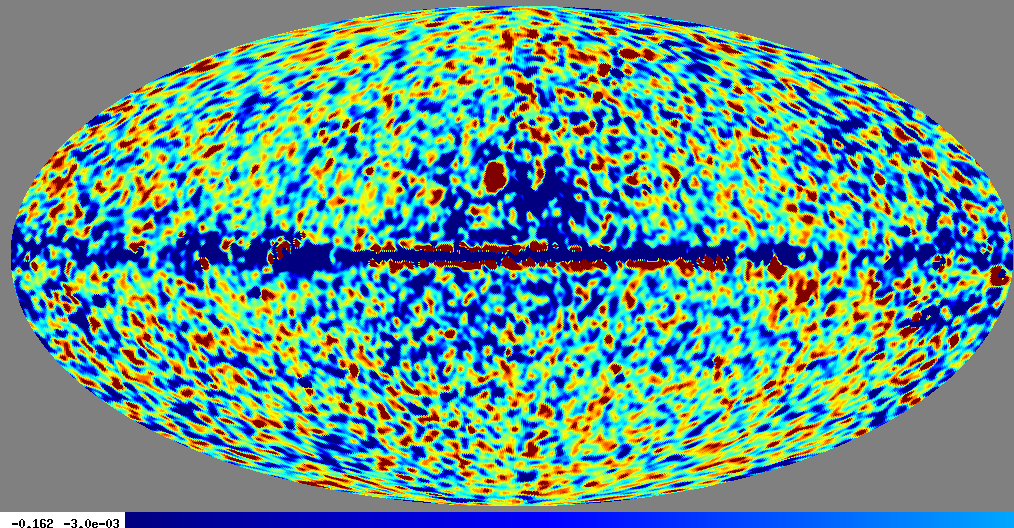
\includegraphics[width=0.40\linewidth]{figures/res_K_exp.png}\\
%        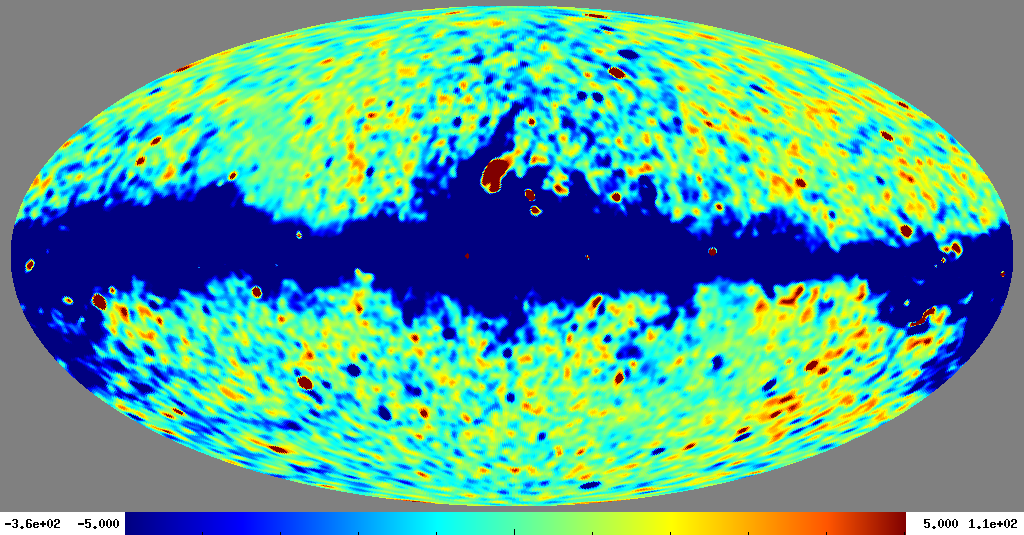
\includegraphics[width=0.40\linewidth]{figures/res_030_spdust.png}
%        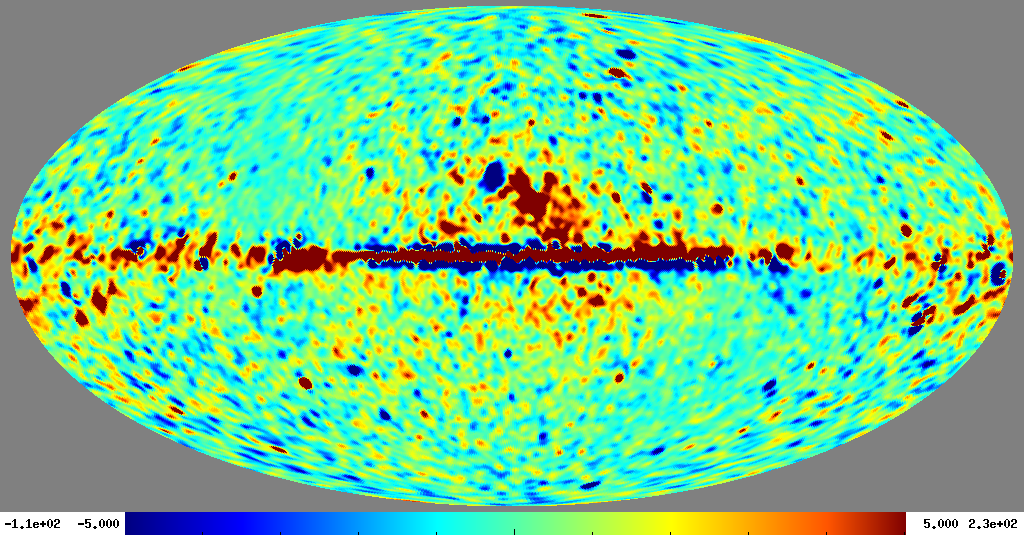
\includegraphics[width=0.40\linewidth]{figures/res_030_exp.png}\\
%        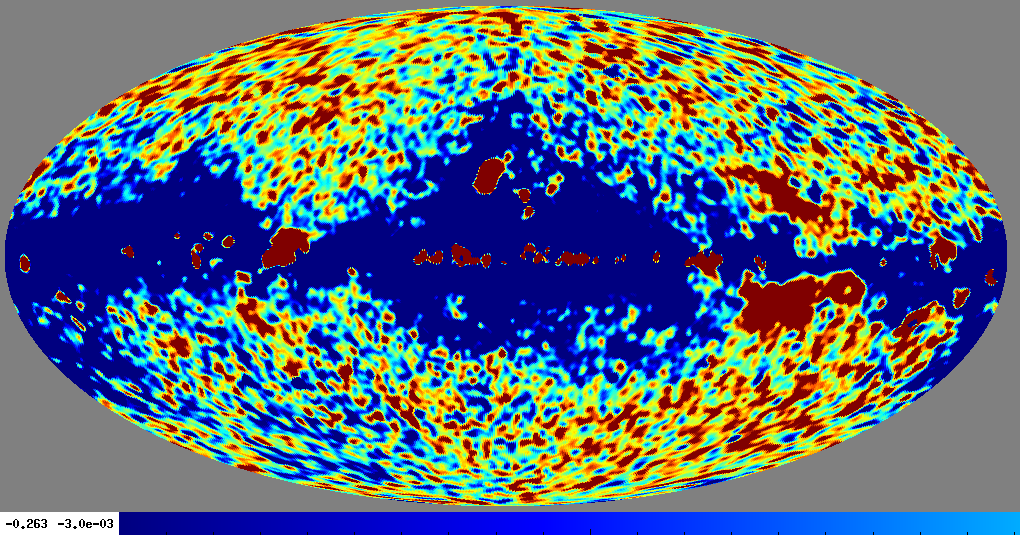
\includegraphics[width=0.40\linewidth]{figures/res_Ka_spdust.png}
%        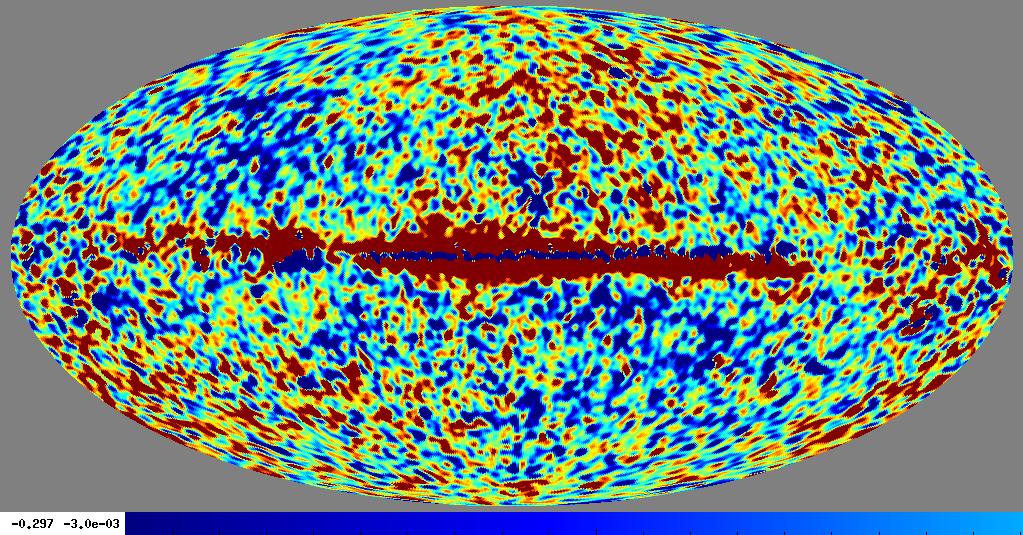
\includegraphics[width=0.40\linewidth]{figures/res_Ka_exp.png}\\
%        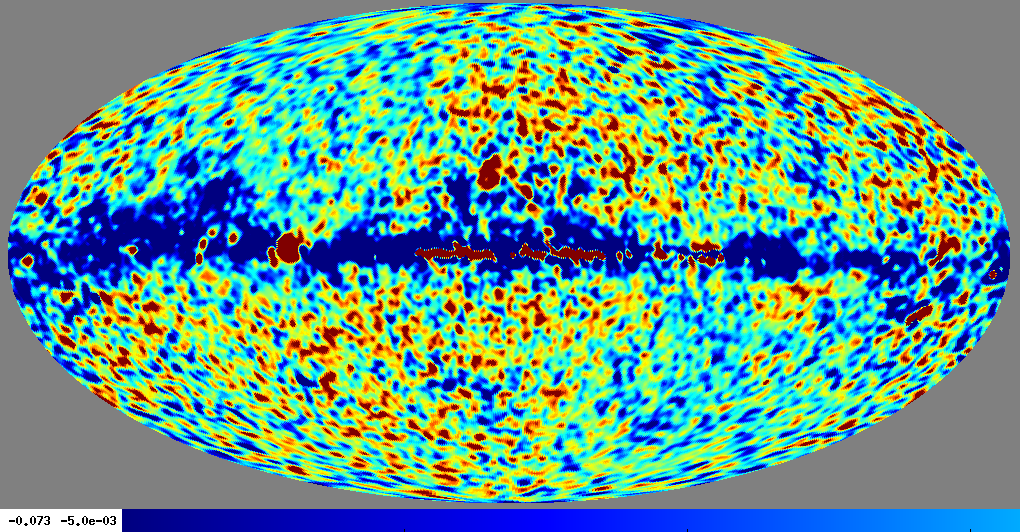
\includegraphics[width=0.40\linewidth]{figures/res_Q1_spdust.png}
%        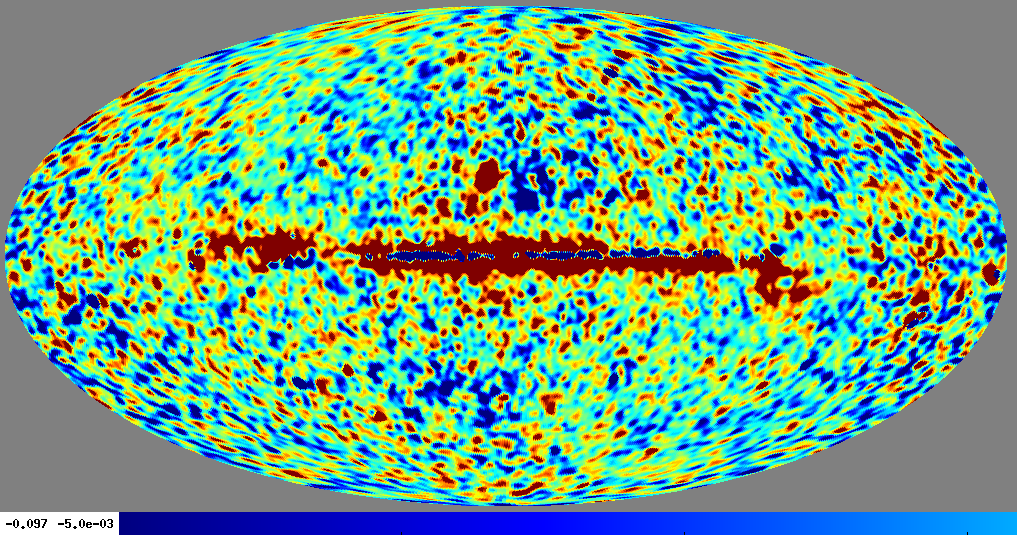
\includegraphics[width=0.40\linewidth]{figures/res_Q1_exp.png}\\
%        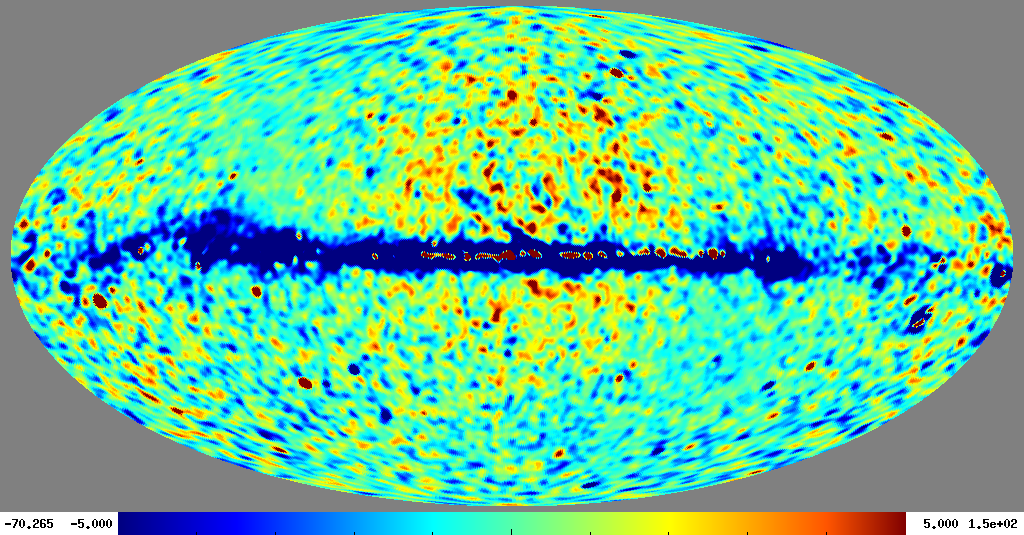
\includegraphics[width=0.40\linewidth]{figures/res_044_spdust.png}
%        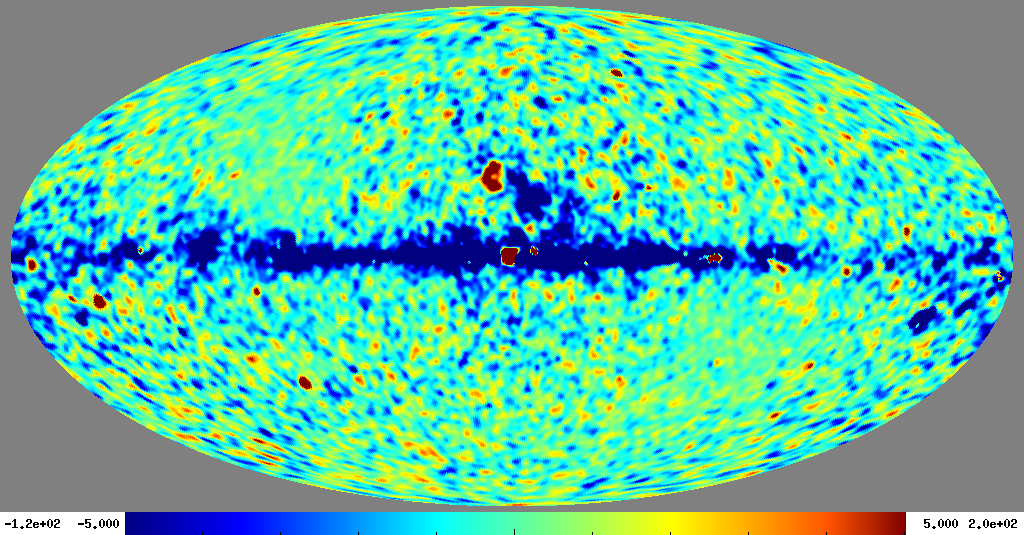
\includegraphics[width=0.40\linewidth]{figures/res_044_exp.png}\\
%        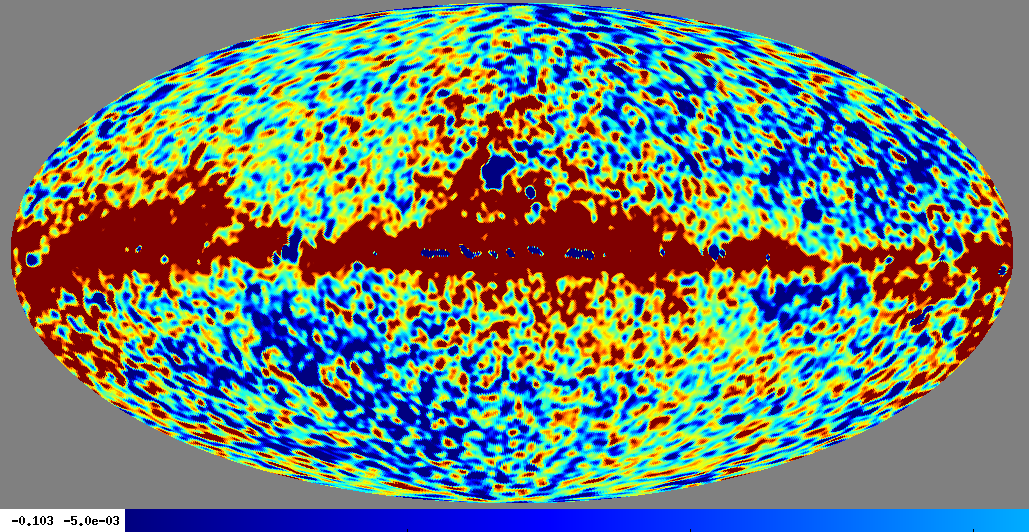
\includegraphics[width=0.40\linewidth]{figures/res_V1_spdust.png}
%        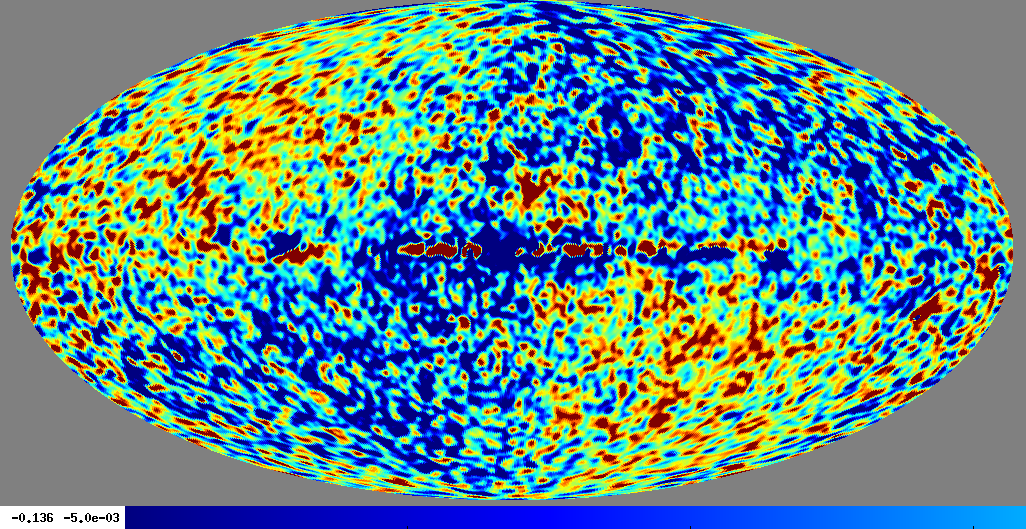
\includegraphics[width=0.40\linewidth]{figures/res_V1_exp.png}\\        
%	\caption{Residuals}
%        \label{fig:residuals}
%\end{figure*}



%We will also use Table 6, Figure (33) of Planck 2018 results IV Diffuse component separation


\subsection{Parametric component estimation}
\label{sec:comm1}

In this section we use \commanderone\footnote{\url{https://github.com/Cosmoglobe/Commander1}} to perform pixel-based component separation on maps smoothed to a common resolution of $5^\circ$ and at $N_\mathrm{side}=64$.\footnote{We use \commanderone\ because it is parallelized over pixels and can quickly determine spatial variation, while \commanderthree\ is optimized for multi-resolution data.}
For this analysis, we perform 100 pixel-based \commanderone\ Gibbs samples on each of the 500 \cosmoglobe\ DR1 Gibbs samples produced by \commanderthree. This allows us to decompose the pure statistical error assuming white noise alone for each of the 100 \commanderone\ samples, while changes between each main DR1 sample show the effects of low-level instrumental processing. In these analyses, we use the same polarized bands as in the main \cosmoglobe\ DR1 analysis, namely \WMAP, \Planck\ LFI, and \Planck\ 353\,GHz. We use a prior $\beta_\mathrm s\sim\mathcal N(-3.1, 0.1)$ for the synchrotron spectral index, while for dust we use a constant spectral index of $\beta_\mathrm d=1.55$ and the dust map $T_\mathrm d$ from \citet{planck2014-a12}.

We used the same data model as in \cosmoglobe\ DR1, but allowed for spatially varying $\beta_\mathrm s$ in two different forms.
First, we allow $\beta_\mathrm s$ to vary over the same regions as in the T-T analysis.
We find that for such large regions, there is very little effect due to the prior, and in particular find a maximum shift of 0.3 between a prior of $\mathcal N(-3.5,0.1)$ and $\mathcal N(-2.7, 0.1)$. We add this difference in quadrature to the uncertainty due to statistical and systematic errors. 
We also compare the reported $\beta_\mathrm s$ maps from QUIJOTE \citep{QUIJOTE_VIII} and CLASS \citep{eimer2023}. We choose these maps because they are to this date the best publicly available synchrotron spectral index maps that are not affected by Faraday rotation off the Galactic plane, as in S-PASS \citep{krachmalnicoff2018,fuskeland:2019}. The delivered $\beta_\mathrm s$ maps are pixelized at $N_\mathrm{side}=64$ and 32, respectively, with associated uncertainty maps taking into account the expected instrumental noise levels. We take an inverse-weighted average of the respective maps and report the weighted standard error within each region, displayed in Fig.~\ref{fig:beta_comp}. 

In general, the uncertainties in our analysis are smaller than each of the other published results, each for slightly different reasons. First, the T-T analyses will inherently have less constraining power than a full likelihood analysis, as this approach only uses two frequency channels via a linear regression, so the uncertainty is determined by the noise level in each frequency channel and the inherent variation within a given sky region. Beyond that, the T-T plot in this paper marginalizes over dependence on the polarization angle $\alpha$, and by design accentuates systematic effects, predominantly beam ellipticity. Finally, the QUIJOTE analysis is most similar in data choice (MFI 11/13\,GHz, \WMAPnine\ \K/\Ka, \Planck\ PR4) and methodology \citep[\texttt{B-SeCRET};][]{b-secret}, but still yields higher uncertainty than the \commanderone\ spectral index region analysis. This is most likely due to different spatial resolution and modeling choices; the \commanderone\ analysis presented here is performed at $5^\circ$ resolution versus the $2^\circ$ resolution per-pixel analysis in \citet{QUIJOTE_VIII}. In addition, \citet{QUIJOTE_VIII} sampled for $\beta_\mathrm d$ and $T_\mathrm{d}$ with priors $\mathcal N(1.55,0.1)$ and $\mathcal N(21,3)$ while using a relatively wide prior on $\beta_\mathrm s$ of $\mathcal N(-3.1, 0.3)$.

At high Galactic latitudes (regions 1--12), there is good agreement between each of the treatments, and all values are consistent with a single constant value. 
In the north and south polar spur (regions 13 and 14) there is excellent agreement between all of the pipelines, while along  the Galactic plane (regions 15--24), there are mild discrepancies between the methodologies, in particular a less distinct amount of periodic structure as a function of Galactic latitude.

\begin{figure}
	\centering
	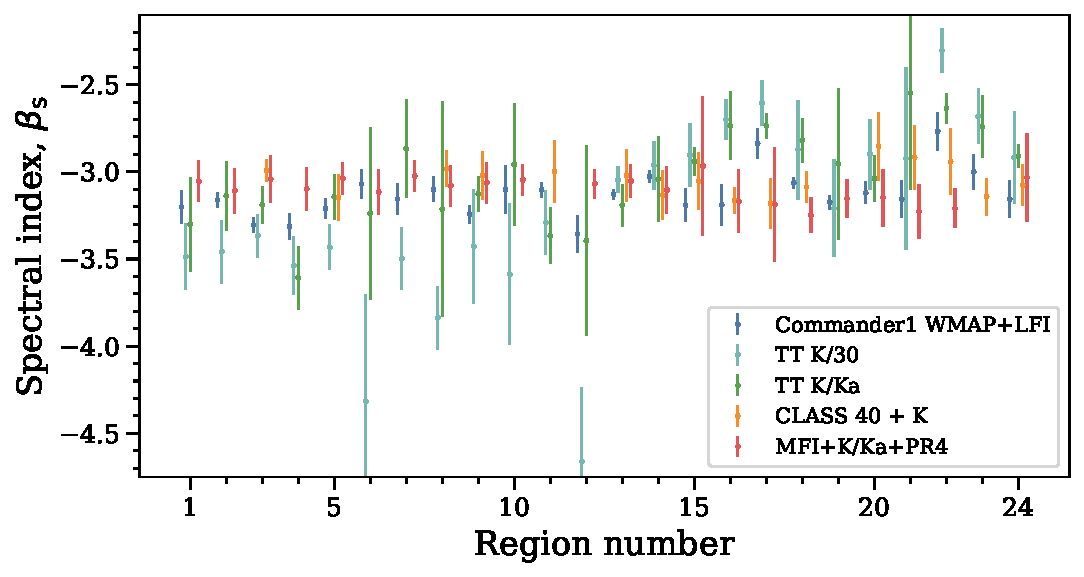
\includegraphics[width=\columnwidth]{figures/compare_betas.pdf}
	\caption{Spectral index from \cosmoglobe\ DR1 spectral index estimation, T-T plots with \K/\Ka, the QUIJOTE estimates, and the CLASS estimates.
	}
	\label{fig:beta_comp}
\end{figure}


To more finely probe the spatial variation of $\beta_\mathrm s$, we perform a second \commanderone\ analysis with identical data and model choices, except the $\beta_\mathrm s$ are allowed to vary with a prior of $\mathcal N(-3.1,0.1)$ and spatially vary along an $N_\mathrm{side}=16$ grid. We found that this was the highest resolution grid in which the spectral index was not prior dominated across all high-latitude regions. In Fig.~\ref{fig:beta_16}, we display the mean of all of the Gibbs samples, along with the standard deviation evaluated per \cosmoglobe\ DR1 Gibbs sample, $\sigma_{\beta_\mathrm s}^\mathrm{stat}$, and the standard deviation over all \cosmoglobe\ DR1 samples and \commanderone\ samples, $\sigma_{\beta_\mathrm s}^\mathrm{sys+stat}$. Put concretely, $\sigma_{\beta_\mathrm s}^\mathrm{stat}$ is the standard deviation when the input maps themselves are static, and $\sigma_{\beta_\mathrm s}^\mathrm{sys+stat}$ includes variations in the frequency maps themselves, corresponding to underlying instrumental effects, including gain, noise characterization, and baseline estimation. The uncertainty due to white noise alone  traces the high signal-to-noise regions of the polarized synchrotron, especially the prominent loops and spurs and the Fan region. At high Galactic latitudes, the standard deviation is 0.1, indicating that the posterior uncertainty is limited by the prior. To further test this, we performed additional \commanderone\ runs with priors of $\mathcal N(-3.2,0.1)$ and $\mathcal N(-3.0,0.1)$, and used the deviation from the mean in the fiducial analysis as an estimate of the extent of prior domination, $\sigma_{\beta_\mathrm s}^\mathrm{prior}\equiv (\langle \beta_{-3.0}\rangle-\langle\beta_{-3.2}\rangle)/2$. Adding this in quadrature gives the total uncertainty, which we display in the bottom panel of Fig.~\ref{fig:beta_16}.

The uncertainty across the entire Gibbs chain does not merely trace high signal-to-noise regions, and in fact there are variations that exceed the prior surrounding the Galactic center. These variations are are primarily due to gain and bandpass uncertainties. It therefore makes sense that gain variations in \K, \Ka, and 30\,GHz around the brightest region of the sky would induce large variations. Despite the relative increase in noise level when including instrumental effects, the brightest Galactic loops, the Cygnus region, and Tau A regions are well-constrained by the data.
In total, there is not enough high-signal-noise data to credibly claim spatial variation in high Galactic latitude regions. 


\begin{figure}
	\centering
	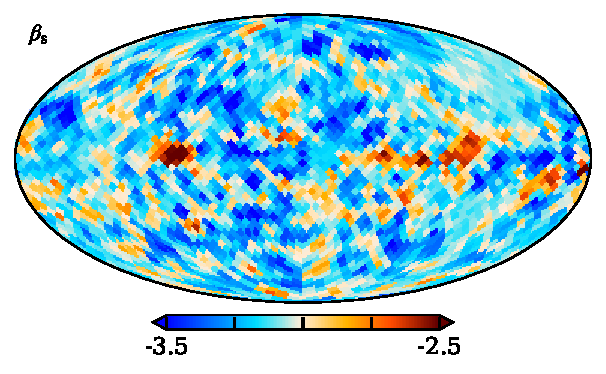
\includegraphics[width=\columnwidth]{figures/beta_n0016_mu.pdf}\\
	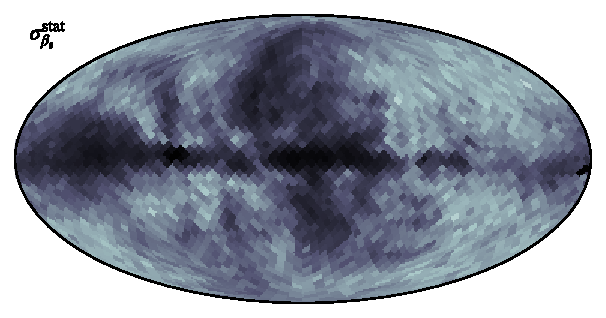
\includegraphics[width=\columnwidth]{figures/beta_n0016_sd_samp.pdf}\\
	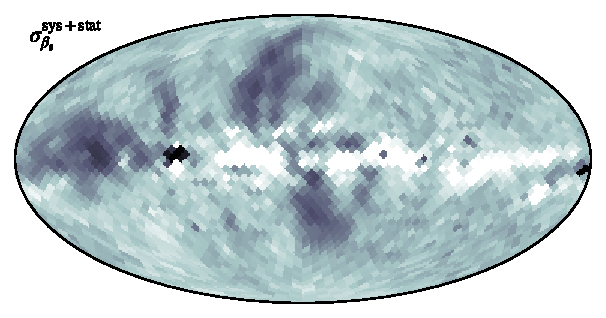
\includegraphics[width=\columnwidth]{figures/beta_n0016_sd_stat_inst.pdf}\\
	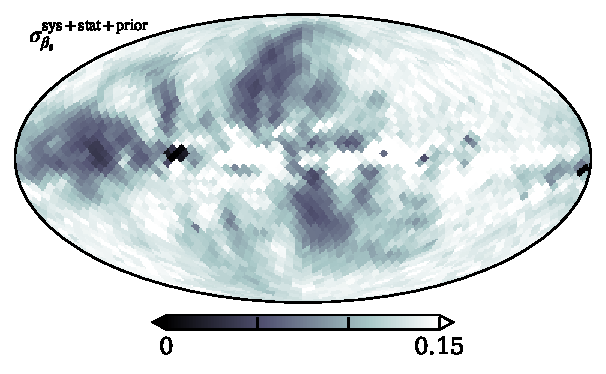
\includegraphics[width=\columnwidth]{figures/beta_n0016_sd_stat_inst_prior.pdf}
	\caption{
		\cosmoglobe\ DR1 $\beta_\mathrm s$ constraints. \textit{(First):} Mean spectral index over all samples, \textit{(second):} standard deviation over a single \cosmoglobe\ DR1 sample, \textit{(third):} standard deviation over all \commanderone\ and \cosmoglobe\ DR1 samples, and \textit{(fourth):} difference due to prior choice added in quadrature.}
	\label{fig:beta_16}
\end{figure}

%Figure .5, seems not useful, as well Figure .4, .3 could go back at the end. .6 can also be taken out


As a final quality check, we display the residuals with respect to the \commanderone\ sky model in Fig.~\ref{fig:res_QU}, as well as the total scaled and normalized $\chi^2$. In all bands but \K, 30\,GHz, and \Ka, there are no visible artifacts due to instrumental uncertainty, with each map showing fluctuations consistent with the estimated white noise level calculated in the DR1 processing.  In addition, many of the residuals visible in Fig.~\ref{fig:cg_residuals} have been reduced, demonstrating that polarized synchrotron spectral index variation provides meaningful improvements to the sky model fit.

The most salient remaining residuals are in \K, 30\,GHz, and \Ka. \K-band and 30\,GHz are anticorrelated surrounding Galactic center, indicating  tension between these two high signal-to-noise datasets. This could either be due to genuine mismodeling of the sky, or be due to incompletely modelled instrumental parameters. In particular, the signature is reminiscent of bandpass leakage corrections, which are shown, e.g., in Fig.~9 of \citet{bp09}.

A more persistent residual is found in the Stokes $Q$ \Ka-band map. This feature has appeared in several different analyses, e.g., Fig.~4 of \citet{bp14} and Fig.~8 of \citet{weiland:2022}, but was not as clear without full removal of the poorly measured modes in the final map. The lack of this feature in the corresponding Stokes $U$ map suggests that the effect is not a true Galactic effect, and is in some way due to instrumental processing, or unmodeled systematics. We discuss potential sources of this signal in Sec.~\ref{sec:conclusion}.

\begin{figure*}
	\begin{center}
	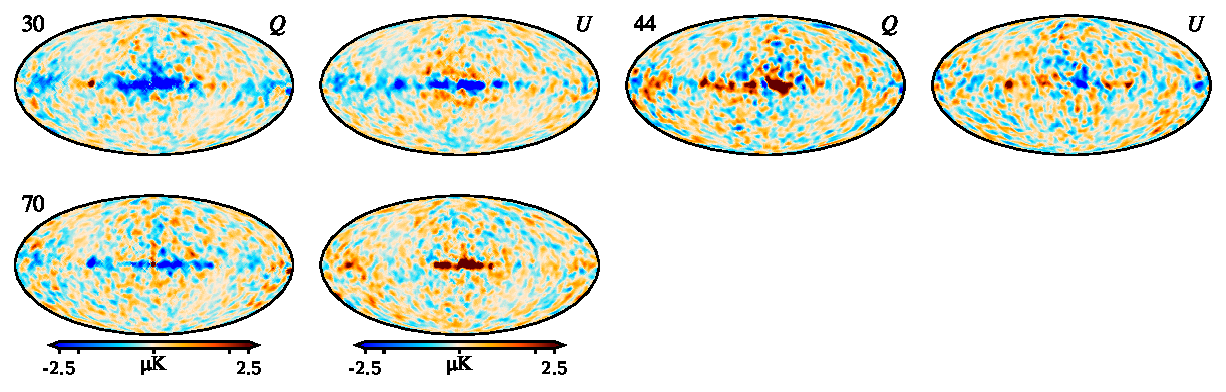
\includegraphics[width=\linewidth]{figures/comm1_res_QU_LFI.pdf}\vspace{-0.3cm}
	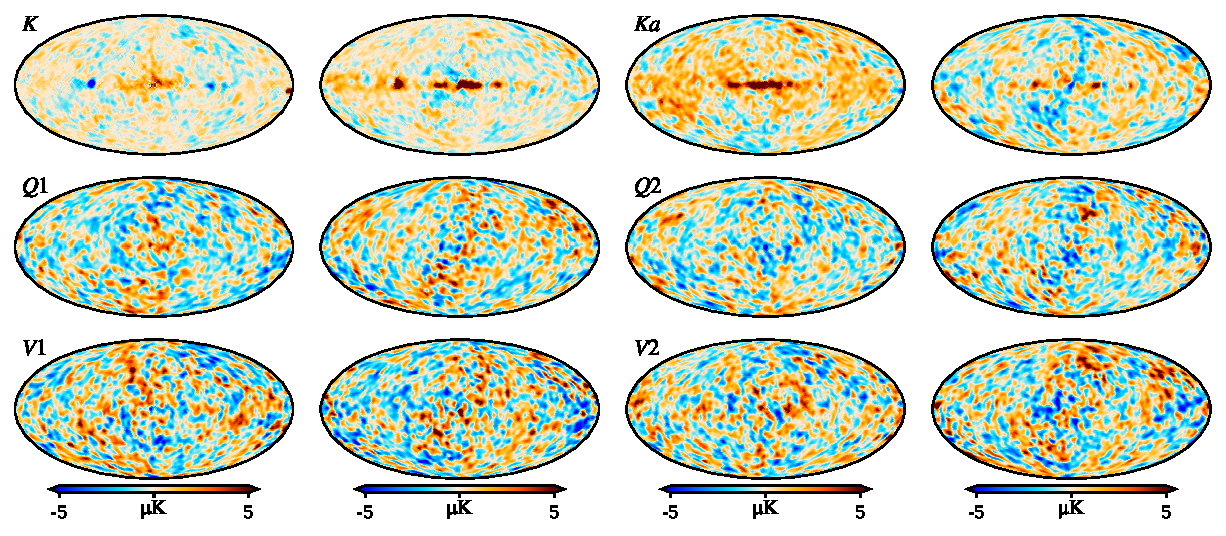
\includegraphics[width=\linewidth]{figures/comm1_res_QU_K-V.pdf}\vspace{-0.3cm}
	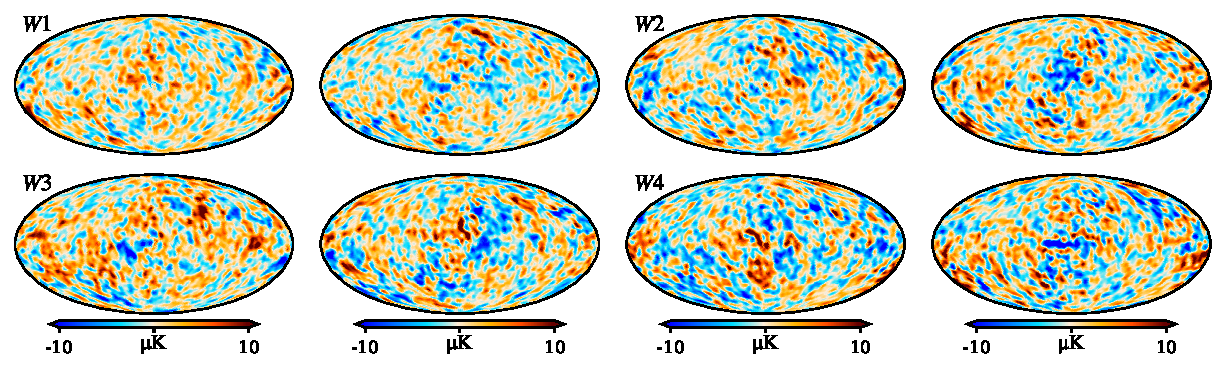
\includegraphics[width=\linewidth]{figures/comm1_res_QU_W.pdf}\vspace{-0.3cm}
	\end{center}\vspace{-0.3cm}
	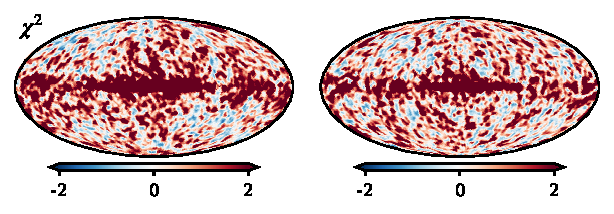
\includegraphics[width=0.5\linewidth]{figures/comm1_res_QU_chisq.pdf}
	\caption{Residual maps and normalized $\chi^2$ for the \commanderone\ analysis of the \cosmoglobe\ DR1 data. Panels are organized with LFI channels in rows 1--2, \WMAP\ in rows 3--7, and the total reduced $\chi^2$ in row 8.}
	\label{fig:res_QU}
\end{figure*}





\section{Discussion and conclusion}
\label{sec:conclusion}

We have presented the state-of-the-art model of polarized synchrotron using the \cosmoglobe\ DR1 data products. The polarized synchrotron map as delivered in \citet{watts2023_dr1} has an effective white noise level of $3.4\,\mathrm{\mu K}$, a 29\,\% improvement over the white noise levels of the \WMAP\ \K-band and LFI 30\,GHz maps. Using the fully consistent reprocessed \WMAP\ and \Planck\ LFI data, we have been able to leverage the full statistical power of both datasets. We have additionally verified that this model characterizes the polarized sky signal to within $5\,\mathrm{\mu K}$ at all bands. We have also reproduced the previously-reported $E$-to-$B$-mode ratio in the polarized synchrotron power spectrum. Furthermore, we have shown that physically reasonable spectral indices can be recovered using a variety of methods, which are consistent with both the methods presented in this paper and with previously published results from CLASS and QUIJOTE, confirming variation in $\beta_\mathrm s$ along the Galactic plane and constant at high Galactic latitudes.


Our improved processing of the \WMAP\ and LFI data in conjunction with improved polarized synchrotron modeling has allowed us to dig deeper into the underlying differences between the two datasets. We have shown agreement between the $\beta_\mathrm s$ values derived using the T-T plot using \K/30\,GHz and \K/\Ka\ data combinations, further evidence that these datasets are now consistent with each other. The remaining unexplained differences between the sky maps and our derived model are primarily in the Galactic center, and have morphologies consistent with bandpass errors and SED complexities.


The least well-understood residual is in the \Ka-band, specifically Stokes $Q$. Of all the known instrumental effects in both \WMAP\ and \Planck\ LFI, the only one that morphologically resembles this residual is the bandpass correction in \K-band, which was previously presented in Figure~12 of \citet{watts2023_dr1}. The bandpass correction term depends solely on laboratory measurements, presented in \citet{jarosik2003:MAP}. The high statistical weight of \K-band for determining polarized synchrotron could easily lead to an undersubtraction in the \Ka-band maps. Conversely, the bandpass correction to \Ka-band itself is negligible, as all of the \Ka-band radiometers were reported to have nearly identical bandpasses. A full accounting of this effect, including sampling of bandpass differences in the \WMAP\ TODs (not performed in \citealt{watts2023_dr1}) will be performed in future work.


The estimation of $\beta_\mathrm s$ is difficult precisely because the quantity is dependent on differences between different frequencies, which can often exacerbate systematic effects and processing choices. The differences between a sky model and datasets is best determined in the timestreams -- much of the improvement demonstrated in this analysis would not have been possible through a purely map-based analysis. Beyond pure improvement of data quality, this approach allowed for a natural end-to-end propagation of errors, and demonstrated that some of the brightest regions of the sky in fact do not have well-determined spectral indices, despite their high signal-to-instrumental noise ratio. As increasingly stringent uncertainty constraints are becoming necessary in order to measure a non-zero tensor-to-scalar ratio, the use of joint information between experiments with complementary observation strategies will increasingly become a necessity. Future joint analysis, including for example QUIJOTE and CLASS data, will continue to improve our knowledge of the polarized sky.


\begin{acknowledgements}
  %We thank Prof.\ Pedro Ferreira and Dr.\ Charles Lawrence for useful suggestions, comments and  discussions. 
  We thank the entire \Planck\ and \WMAP\ teams for
  invaluable support and discussions, and for their dedicated efforts
  through several decades without which this work would not be
  possible. The current work has received funding from the European
  Union’s Horizon 2020 research and innovation programme under grant
  agreement numbers 819478 (ERC; \textsc{Cosmoglobe}) and 772253 (ERC;
  \textsc{bits2cosmology}).
  In
  addition, the collaboration acknowledges support from
  RCN (Norway; grant no.\ 274990).
  We acknowledge the use of the Legacy Archive for Microwave Background Data
  Analysis (LAMBDA), part of the High Energy Astrophysics Science Archive Center
  (HEASARC). HEASARC/LAMBDA is a service of the Astrophysics Science Division at
  the NASA Goddard Space Flight Center.  
  Some of the results in this paper have been derived using the \texttt{healpy}
  and \texttt{HEALPix}\footnote{\url{http://healpix.sf.net}} packages
  \citep{gorski2005, Zonca2019}.  This work made use of
  Astropy:\footnote{\url{http://www.astropy.org}} a community-developed
  core Python package and an ecosystem of tools and resources for
  astronomy \citep{astropy:2013, astropy:2018, astropy:2022}.
\end{acknowledgements}


\bibliographystyle{../../common/aa}

\bibliography{../../common/Planck_bib,../../common/CG_bibliography}

\begin{appendix}

\section{T-T Plots}
\label{sec:appendix}

\noindent\begin{minipage}{\textwidth}
	This section shows two intermediate results in the T-T plot analysis. Figure~\ref{fig:cos30_beta_bigscatter} shows the scatter plots within each individual region for both the \WMAPnine\ and \cosmoglobe\ DR1 results, while Fig.~\ref{fig:cos30_beta_bigalpha} shows the measured spectral index as a function of polarization angle $\alpha$. For more details, the interested reader can consult \citet{fuskeland2014}.
\end{minipage}

\noindent\begin{minipage}{\textwidth}
\vspace*{1mm}
\centering
%\hspace*{1.5cm}
\includegraphics[width=0.9\linewidth]{figures/ut_big_multiscatterplot_converted.pdf}
\captionof{figure}{T-T plots for Stokes $Q$ and $U$ maps of the \Cosmoglobe\ DR1 \K-band versus the \Cosmoglobe\ DR1 30\,GHz (black) and the \WMAPnine\ \K-band versus \Planck\ PR3 30\,GHz (red) for all regions. The horizontal (solid and dotted) lines indicate the corresponding inverse variance weighted values of the spectral index, averaged over rotation angle, and in the \Cosmoglobe\ case also weighted over samples.}
\label{fig:cos30_beta_bigscatter}
\label{fig:baseline}
\end{minipage}

%\begin{figure*}
%        \centering
%        %\includegraphics[width=\linewidth]{figures/ut_big_multiscatterplot.eps}
%        \includegraphics[width=0.95\linewidth]{figures/ut_big_multiscatterplot_converted.pdf}
%        \caption{T-T plots for Stokes Q and U maps of the \Cosmoglobe\ \K-band versus the \Cosmoglobe\ 30\,GHz (black) and the \WMAPnine\ \K-band versus \Planck\ 2018 30\,GHz (red) for all regions. The horizontal (solid and dotted) lines indicates the corresponding inverse variance weighted values of the spectral index, averaged over rotation angle, and in the \Cosmoglobe\ case also samples.}
%        \label{fig:cos30_beta_bigscatter}
%\end{figure*}

%\noindent\begin{minipage}{\textwidth}
\begin{figure*}
        \centering
        %\includegraphics[width=\linewidth]{figures/cos30_ut_big_multialphaplot.eps}
        \includegraphics[width=0.9\linewidth]{figures/cos30_ut_big_multialphaplot_converted.pdf}
        \caption{Synchrotron spectral index as a function of rotation angle, computed using T-T plot between the \Cosmoglobe\ DR1 \K-band and the \Cosmoglobe\ DR1 30\,GHz (black) compared to the spectral index using the \WMAPnine\ \K-band and \Planck\ PR3 30\,GHz (red) for all regions. The horizontal (solid and dotted) lines indicates the corresponding inverse variance weighted values of the spectral index, averaged over rotation angle, and in the \Cosmoglobe\ case also samples.}
        \label{fig:cos30_beta_bigalpha}
\end{figure*}
%\end{minipage}

\end{appendix}

\end{document}
